% fithesis2 with modifications used, please use local fithesis.cls file, not system-wide installed.
\documentclass[11pt,oneside,final]{fithesis2}
% \documentclass[oneside,final]{fithesis2}
% \usepackage[resetfonts]{cmap}
\usepackage{lmodern}

\usepackage[english]{babel}
\usepackage[utf8x]{inputenc}
%\usepackage[IL2]{fontenc}
\usepackage[T1]{fontenc}

\usepackage{hyperref}
\usepackage{graphicx}
\usepackage{color}
\usepackage{afterpage}
\usepackage{calc}
\usepackage{subfig}
\usepackage{amssymb}
\usepackage{amsthm}
\usepackage{amsmath}
\usepackage{enumitem}
%\usepackage{titlesec}

% floating for figures H
\usepackage{float}
\restylefloat{figure}

% \usepackage{sistyle}

% some symbols in package
% \usepackage{textcomp}
% \usepackage{inputenx}

% text super/sub scripts
\usepackage{fixltx2e}

% % algpseudocode was not installed by default; http://ctan.org/pkg/algorithmicx
% % http://tex.stackexchange.com/questions/38978/how-can-i-manually-install-a-latex-package-debian-ubuntu-linux
% % http://ftp.cstug.cz/pub/tex/CTAN/macros/latex/contrib/algorithmicx/algorithmicx.pdf
\usepackage{algpseudocode}

% \usepackage[options]{algorithm2e}
\usepackage{algorithm}
%\usepackage{algorithmic}

% nicefrac
\usepackage{units}



\def\R{\mbox{\sffamily\bfseries R}}

\DeclareGraphicsExtensions{.pdf,.png,.jpg,.gif}

\thesislang{en}
\thesistitle{Cryptography in an untrusted environment}
\thesissubtitle{Diploma thesis}
\thesisstudent{Dušan Klinec}
\thesiswoman{false}
\thesisfaculty{fi}
% \thesiswords{slov: 628}
% \thesisstudentuco{UČO: 325219}
\thesisyear{2013}
\thesisadvisor{RNDr.\,Petr Švenda,\,Ph.D.}

\newcommand{\reci}[1]{\frac{1}{#1}}
\newcommand{\hypot}[2]{\sqrt{#1^2+#2^2}}
\newcommand{\cbrt}[1]{\sqrt[3]{#1}}

% protocols & commands
\newcommand{\comproto}[1]{\emph{#1}}
\newcommand{\protocommand}[1]{\emph{\uppercase{#1}}}
\newcommand{\protoparam}[1]{\emph{#1}}
%\underset{x}{\operatorname{argmin}}

% some math & modulo
\newtheorem{mydef}{Definition}
\newtheorem{myprop}{Proposition}
\newtheorem{mytheorem}{Theorem}
\makeatletter
\def\imod#1{\allowbreak\mkern10mu({\operator@font mod}\,\,#1)}
\makeatother

\newcommand{\gfe}{\ensuremath{\text{GF}\left(2^8\right)}}
\newcommand{\gf}{\ensuremath{\text{GF}\left(2\right)}}

% bibtex
% Czech bibtex citation norms
% http://www.abclinuxu.cz/blog/Drobnosti/2007/3/csplainnat.bst-nbsp-cesky-styl-pro-bibtex-dle-iso-nbsp-690
% svn://kraken.pedf.cuni.cz/csplainnat/
% http://www.fit.vutbr.cz/~martinek/latex/czechiso.html.cs.iso-8859-2
% http://repo.or.cz/w/csplainnat.git
% http://www.root.cz/clanky/odborny-text-v-lyx-matematika-a-bibliografie/nazory/418552/
\usepackage{url}
\usepackage[numbers]{natbib}
\bibliographystyle{unsrtnat}

\usepackage{fancyhdr}
\pagestyle{plain}

% multi-row
\usepackage{multirow}
\usepackage{color, colortbl}

\definecolor{Gray}{gray}{0.85}
\newcommand{\clg}{\cellcolor{Gray}}
\newcommand{\eal}{\emph{et~al.}}

% \fancyhead[LE,RO]{\slshape \rightmark}
% \fancyhead[LO,RE]{\slshape \leftmark}
% \fancyfoot[C]{\thepage}


\hyphenation{how-to}

\begin{document}


\newenvironment{atribut_description}
{\begin{description}
  \renewcommand{\makelabel}[1]{\texttt{\hspace{6pt}##1 $-$}}%
  \setlength{\itemsep}{1pt}
  \setlength{\parskip}{0pt}
  \setlength{\parsep}{0pt}}
{\end{description}}
\renewcommand{\tiny}{\fontsize{7.7}{9.7}\selectfont}

\FrontMatter
\ThesisTitlePage

% BEGINNING OF THESIS ASSIGNEMENT
% % \begin{alwayssingle}
% % 	\afterpage{
% % 	\clearpage
% % 	\begin{figure*}[ht!]
% 	\begin{center}
% 	\leavevmode
% 	\scalebox{1.00}{\includegraphics[trim=100 100 100 40]{bpThesisAssignement_corr.pdf}}
% 	\end{center}
% % 	\caption{Pôdorys študovne so vzdialenosťami objektov \cite{img_skm_studyroom}}
% % 	\label{fig:studyroom_distances}
% % 	\end{figure*}
% %  	}
% %  	\afterpage{\clearpage}
% % \end{alwayssingle}
% END OF THESIS ASSIGNEMENT

\begin{ThesisDeclaration}
\DeclarationText
\AdvisorName
\end{ThesisDeclaration}

\begin{ThesisThanks}
[TODO] Thanks here
\end{ThesisThanks}

\begin{ThesisAbstract}
[TODO] Abstract here
\end{ThesisAbstract}

% BEGINING OF ENGLISH ABSTRACT
% \begin{alwayssingle}
% \chapter*{\AbstractTitleen}
% \par\vfil\null
% \end{alwayssingle}
% \newpage
% END OF ENGLISH ABSTRACT
 
\begin{ThesisKeyWords}
white box attack resistant cryptography, look up tables form, AES
\end{ThesisKeyWords}
\MainMatter
\renewcommand{\contentsname}{Table of contents}

\tableofcontents

% with this - there are no decorative lines in page header
%\pagestyle{plain}

\chapter{Introduction}
%     [TODO] Introduction here
%     Classic ciphers, authentication protocols. Now study of computing in untrusted environment.
    
%     The development and recent advances in 
    
    In the last few decades we have been witnessing a development in a field of outsourced computations and storage.
    The rising prevalence of this computing model slightly changes the classical attacker model 
    that cryptography used to dealt with, what gave rise to a \emph{mobile cryptography}.

    %The classical cryptography address
    The classical goals the cryptography addresses~are confidentiality, data integrity, authentication~and non-repundation~\citep{Menezes:1996:HAC:548089}.
    From the data confidentiality perspective the typical scenario is two remote parties, Alice and Bob, want to communicate via untrusted channel, while the 
    computations on both sides are considered as trusted, an potential attacker resides in a communication link.
    A bunch of cryptography primitives addressing security issues in this scenario
    was invented, analyzed and widely used, like symmetric and asymmetric cryptosystems, digital signatures, authentication protocols, etc...
    
    But with the expansion of out-sourced computations and storage we are getting to a situation that Alice does not trust even to Bob, but wants 
    to use Bob's resources for her purpose. Such outsourcing rises concerns about the loss of a privacy of private data what poses the potential
    barrier in adopting cloud services widely. To ensure the privacy, data is encrypted. The major problem with this model 
    is that in order to evaluate a function over data, e.g. searching in an encrypted database, data has to be decrypted first. This poses another additional 
    overhead. \emph{Fully homomorhpic encryption} provides a solution for these issues.
    
    Another major part of uses cases is the protecting a private function computed in an untrusted environment. Typical example
    of the function to be protected is the license code verification embedded in software or it is a software that provides access 
    to some protected material.  The major goal is to protect these
    functions from analysis, tampering or extraction of a cryptographic material. Software protection techniques like \emph{obfuscation}
    addressing these issues are used in practice. This thesis is devoted to a \emph{whitebox cryptography}, the field of 
    cryptography that studies the level of security of cryptographic algorithms executed in untrusted environment.

    This thesis studies in particular transformation of the AES cipher \citep{2002-daemen} implementation in a such way they provide some
    level of security when executed in untrusted environment. This transformed implementation has embedded symmetric key inside
    and the main goal of the transformation is to resist practical attacks attempting its extraction. Thesis covers introduction
    to whitebox cryptography, describes first such transformation published together with cryptanalysis. It also analyzes the new 
    proposed transformation that should resist key extraction. The thesis states also a proof that this scheme can be broken 
    using already existing attack. In the end some improvements are suggested.

    Chapter 2 describes mobile cryptography concepts and current state of the art in this field mainly with focus on obfuscation and homomorphic encryption.
    In chapter 3 the whitebox cryptography is introduced, explaining the basic building blocks used for transformations. The first proposed scheme 
    by Chow~\eal~\citep{Chow02white-boxcryptography} is described in detail together with the following cryptanalysis by Billet~\eal~\citep{Billet:2004:CWB:2080787.2080809}.
    Chapter 4 covers new whitebox scheme for AES by Karroumi~\citep{Karroumi:2010:PWA:2041036.2041060} in a detail. 
    Description of the schemes and attack implementation follows. 
    In chapter 5 improvements for whitebox schemes are proposed together with their analysis. The last two chapters are devoted to possible further 
    research directions and conclusion.

    I declare this thesis is my own work, but I consulted the problems and proposed solutions together with people from laboratory of security, 
    faculty of Informatics form Masaryk University, and from this reason is personal pronoun ``we'' used instead of ``I''.

\chapter{Area overview}\label{sec:theory}
    
    \section{Overview}
    %[TODO] Overview, setting picture in cryptographic world
    Computing in an untrusted environment is closely related to the notion of \emph{mobile cryptography} \citep{mobile_cryptography} which was established 2 decades ago.
    It analyzes the security problems raised by the concept of mobility of the executable code. The executable code that acts autonomously on behalf a user in collecting 
    and processing information is denoted as a \emph{mobile agent}. Mobile cryptography mainly studies the two security threats.
    \begin{enumerate}
     \item protection of the host from malicious mobile code
     \item protection mobile code from the malicious host
    \end{enumerate}
    
    The former threat can be mitigated to a acceptable level with countermeasures like sandboxing/virtualization and code signing. The latter is much difficult to address 
    and even after 20 years there are no satisfactory techniques to achieve acceptable protection of the code executed on malicious host for a reasonable price.
    
    The problem can be solved by using tamper resistant hardware such as cryptographic smart cards. With a device that acts as an oracle it is possible to achieve some
    level of protection but assumption that such hardware is widely available is false in general, what leads to ideas based on cryptographic primitives.
    
    \section{Obfuscation}
    
    \emph{Obfuscation} is another technique addressing the same problem. Roughly speaking, the major principle is the transformation of the code to a form that is very difficult 
    to analyze and to modify. The potential attacker should not be able to gain any knowledge from the running program, in the ideal case, while the same functionality 
    of the program is preserved. Barak~\eal~formalized the notion of obfuscation in \citep{Barak:2012:POP:2160158.2160159}, providing result that it is impossible 
    to create a generic obfuscator by showing family of functions that are unobfuscatable, i.e. the family of functions always leaking some information. On the other hand
    later was published first positive result \citep{Lynn04positiveresults} claiming it is possible to construct some provably secure obfuscators for point functions.
    It was used to obfuscate complex access control functionalities.
    
    In practice the obfuscators are used widely as a software protection technique that provides some level of protection from attackers but it lacks some 
    security proof so it is preferable to use some cryptographic primitives that has been proven secure. 
    
 %   \section{Computing with encrypted data/functions}
\section{Homomorphic encryption}
    The idea oh homomorphic encryption comes from 
    

    \begin{enumerate}
     \item cloud motivation
     \item computing with encrypted data / functions
     \item multiparty schemes using interaction
     \item converting arbitrary function to network of boolean functions (or addition/multiplication)
	\begin{enumerate}
	 \item depth of the circuit
	 \item universality vs. depth restriction
	\end{enumerate}
    
%     \section{Mobile cryptography}
%     [TODO] Motivation for white box cryptography
%     \begin{itemize}
%      \item computation with encrypted data
%      \item computation with encrypted function
%     \end{itemize}
%
%    \section{Homomorphic encryption}
%     [TODO] Homomorphic encryption follows computation with encrypted data function.
%    Motivation: cloud computation. Short history, recent state of the art...
    
    
     \item simple schemes - GCD, somewhat homomorphic scheme, bootstraping, noise
     \item summarize 3 different approaches (integer lattice, approximate GCD, learning with errors)
     \item special somewhat schemes (unlimited addition, limited multiplication, uses)
     \item new advances in 2010--2012, noise reduction techniques, modulus switching
     \item SIMD execution with Chineese Remainder Theorem, slots of plaintext in ciphertext, cyclotomic ring of polynomials
     \item practical usability, homomorhpic AES implementation
     \item state of the art practical results - numbers, key, running time
    \end{enumerate}

\chapter{Whitebox cryptography}
    
    \section{Introduction}    
% Whitebox def
    In this part of a cryptography we are studying the cryptographic algorithms with a~much stronger attacker model, saying it is executed in a~whitebox context. 

% attacker def
    \emph{Whitebox context} (also abbreviated as WBC) is itself defined by the attacker model, which was introduced by Chow \emph{et~al.} \citep{Chow02white-boxcryptography} in 2002.
    An WBC attacker has full control over execution of the particular algorithm. Namely attacker has the following abilities:
    
    \begin{itemize}
	\item can observe execution:
	\begin{itemize}
	    \item access to the instructions processing at the moment of the computation
	    \item trace the algorithm flow
	    \item sees the memory used
	\end{itemize}
	\item controls the execution environment - runtime modification:
	\begin{itemize}
	    \item tamper the program memory
	    \item execute only a specified part of the algorithm (one round of the cipher)
	    \item modify if-conditions
	    \item change a cycle counters
	    \item fault induction
	\end{itemize}
    \end{itemize}
    
    It is in contrast to \emph{blackbox context} (also abreviated as BBC), the standard cryptographic model, where attacker has only access to the output of the cryptographic algorithm. 
    In BBC the cryptographic algorithm is considered as an oracle/blackbox evaluating some function (analogy to executing algorithm in secure environment).
    Depending on a finer granularity of an attacker model, one can have 
    access only to an algorithm output (ciphertext), or attacker can also query an oracle (chosen plain-text attack) and so on, but has no access to computation itself.

    The cryptographic algorithms (we are mainly interested in symmetric ciphers in this thesis) were extensively studied for attacks in BBC in past.
    They were originaly designed to resist attacks considering only BBC. But if the context is wrong, it can be possible entry point for an attacker.
    Typical example is DRM \footnote{Digital rights management, \textless\url{http://en.wikipedia.org/wiki/Digital_rights_management}}, where software of a~vendor
    (representing the rights owner) is executed in potentially hostile environment, where user can have motivation to extract protected content without
    restrictions added by DRM software. In this situation we cannot consider DRM software to be executed in BBC.
    
    Let's take some symmetric block cipher as an another example. Usually it is constructed as a~keyed permutation (round function) that is repeated 
    several times to add randomness and to improve statistical results of the cipher, increasing security. But if we can inspect such execution, it is 
    very easy to extract encryption keys, since we can read memory during execution or trace algorithm flow.
    
    One such whitebox attack is \emph{Key Whitening Attack} \cite{Kerins06acautionary}. Key whitening is technique intended to increase the security of the iterated block cipher.
    It is typically implemented as adding a~key material to the data (usually by simple operation, such as XOR) in the first and the last round. Such key whitening 
    is used by Twofish \citep{Schneier98twofish:a} and in modified version (only adding the key material in the last round) also AES \citep{2002-daemen}. In Key Whitening Attack
    cipher's binary is modified (we are in whitebox context) in such a~way that the output of the cipher will be the key material itself. 
    
    The main goals of a~whitebox attack is to extract a~key material (usually the symmetric key) or to build an inverse cipher i.e. perform decryption 
    with tables for encryption with a~embedded key.
    
    The definition of whitebox cryptography could be:
    ``The challenge that white-box cryptography aims to address is to implement a~cryptographic algorithm in 
    software in such a~way that cryptographic assets remain secure even when subject to white-box attacks.
    Software implementations that resist such white-box attacks are denoted white-box implementations.'' \cite{hiding_keys}.
    
    \section{History}
    % History overview, oorschot, billet, imposibility of obfuscation, generic attacks on AES, DES
    
    The whitebox cryptography is a quite new field of cryptography. The study of the whitebox implementation of the ciphers started by first 
    whitebox implementation of AES \citep{Chow02white-boxcryptography} and DES \citep{Chow02awhite-box} by Chow~\eal~in~2002. 
    
    At first the cryptanalysis of DES focused on simplified variant of DES. The first published in 2002 by Jacob~\eal
    uses fault injection \citep{conf/ccs/JacobBF02}, another one published in 2005 by Link\eal. uses statistical analysis \citep{Link:2005:COI:1058430.1059147}.
    Later cryptanalysis of fully encoded variant of DES was published by Wyseur~\eal~in~2007 using truncated differentials.
   
    The similar case is AES. Two years after publishing whitebox AES scheme the successful cryptanalysis \citep{Billet:2004:CWB:2080787.2080809} was
    published by Billet~\eal~that enabled to recover embedded symmetric 
    key in less that $2^{30}$ steps. Later in 2008 the generalized version of the previous attack
    was published \citep{Michiels:2007:MST:1314276.1314291} by Michiels~\eal~affecting the larger family of ciphers using the same structure as AES.   
   
    There were also attempts to fix whitebox AES scheme by adding additional linear mappings and increasing size of the implementation in \citep{XiaoLai}
    as a~response to the Billet's attack.
    The attack using linear equivalence algorithm was published in 2012 \cite{conf/sacrypt/MulderRP12}.
    
    The another attempt how to fix whitebox AES was introducing random perturbations \citep{journals/iacr/BringerCD06a}, 
    complicating algebraic cryptanalysis but the effective attack was published by Mulder~\eal \citep{conf/indocrypt/MulderWP10}.
    
    Last not least a whitebox AES scheme using dual ciphers \citep{Karroumi:2010:PWA:2041036.2041060} was published in 2011. The paper claimed 
    the scheme is robust enough to resist practical attacks on the implementation what we proved is false. 
    Thesis is mainly focused on this scheme, what is generalization of the first whitebox AES scheme. 
    

    \section{Whitebox AES scheme}
    % Schemes used with AES, DES. Some techniques used in whiteboxing the cipher (input output encodings, mixing bijections - diffusion layers)

    The first whitebox AES implementation, published by Chow~\eal~\citep{Chow02white-boxcryptography} is based on the look-up tables implementation, that was also
    mentioned in original AES paper \citep{2002-daemen}. Note that it is easy to transform AES cipher with embedded encryption key 
    to a~network of look-up tables and to use these computed tables for encryption (or decryption). But this implementation is vulnerable in whitebox context,
    since it is possible to extract encryption key with algebraic analysis of the look-up tables, recall all building blocks (except key schedule) of AES are key-independent 
    and publicly available. Thus these look-up tables has to be further protected to resist algebraic attacks. 
    
    We are mainly focused on AES-128, for simplicity but the same strategy can be applied also to AES-256.

    For further explanation we will need the following definitions:

    \begin{mydef}\label{def:linear_mapping}
    Linear mapping is mapping $L\left(x\right)$ over $\text{GF}(2)^n$ that satisfies $\forall \; x,y \in \text{GF}(2)^n \; : \; L(x+y) = L(x) + L(y).$
    \end{mydef}
    
    \begin{mydef}\label{def:affine_mapping}
    Affine mapping is mapping $A(x)$ over $\text{GF}(2)^n$ such that $A(x) = L(x) + c, c \in \text{GF}(2)^n$ and $L(x)$ is linear mapping.
    \end{mydef}

    \subsection{AES-128}
    The brief introduction of AES is required for further understanding of whitebox implementation and implementation based on dual AES in section \ref{sec:wb_dual_aes_sec}.
    
    AES-128 is a~symmetric, iterated, block cipher that maps $128 \rightarrow 128$ bits (block length) using a 128-bit encryption key. It has 10 rounds and operates
    over $4\times4$ byte array. AES works with $\gfe$ and operations used in AES have quite algebraic nature. For each round is generated a key material called round keys
    by key-schedule routine from encryption key. 
    
    The key-schedule is not important operation from our perspective and can be abstracted in further explanations. Important fact about the key-schedule is it is reversible i.e. 
    if we have round keys from 2 consecutive rounds it is possible to derive all other round keys, even the encryption key (the encryption key is used as round key in the first round).
    
    Besides the key-schedule there are 4 operations used in main AES body:
    \begin{itemize}
     \item \emph{AddRoundKey} adds round keys to the state array. It is simple XOR of two $4\times4$ byte arrays.
     \item \emph{ShiftRows} performs a simple shift of each row of the state array to the left, by the row index (indexing from 0).
     \item \emph{SubByte} is $8 \rightarrow 8$ bijection, the only non-linear operation, performing 
	\emph{confusion}\footnote{\emph{Confusion} is a~property of secure cipher defined by Shannon \citep{shannon-otp}, it should make relation between ciphertext and symmetric encryption
	    key complex.}. It uses inversion in $\gfe$.
     \item \emph{MixColum} is the main \emph{diffusion}\footnote{\emph{Diffusion} is a~property of secure cipher defined by Shannon \citep{shannon-otp}, it should make relation between
	    ciphertext and plaintext complex, dissipating small change into large range. Diffusion contributes to the avalanche effect. } operation. It corresponds to a matrix multiplication in $\gfe$. 
	    State array column is multiplied from left by MixColumn $4 \times 4$ matrix (also denoted as MC). Due to this operation after one round of the cipher, 
	    one byte of the state array depends on 4 bytes of the input state array.
    \end{itemize}
    
    \subsection{AES table implementation}\label{sec:aes_table}
    Algorithm \ref{alg:AESalg} is AES in a~form suitable for whitebox implementation, i.e. some operations were regrouped in such a~way that round keys addition 
    is right before \emph{SubByte} operation. This enables to merge these two operations to one $8\times8$ look-up table as is described in equation \ref{eq:tboxes}.
    Resulting tables following this construction are called T-boxes.
    
    \begin{subequations} \label{eq:tboxes}
    \begin{align}
	T^r_{i,j}(x)    &= S\left(x \oplus k^r_{i,j}\right)\\
	T^{9}_{i,j}(x)  &= S\left(x \oplus k^{9}_{i,j}\right) \oplus k^{10}_{i,j}
    \end{align}
    \end{subequations}

    \begin{algorithm}
        \caption{AES algorithm, form suitable for whitebox implementation}
	\begin{algorithmic}[1]
	    \Function{AES}{$plaintext, k$}  \Comment{k is array of round keys}
	    \State $state \gets plaintext$          \Comment{state is $4 \times 4$ byte array}
	    \For{$r\gets 0, $ to $8$}
		\State $\text{ShiftRows}(state)$
		\State $\text{AddRoundKey}(state, k_{r})$
		\State $\text{SubByte}(state)$
		\State $\text{MixColumn}(state)$
	    \EndFor
	    \State $\text{ShiftRows}(state)$
	    \State $\text{AddRoundKey}(state, k_{9})$
	    \State $\text{SubByte}(state)$
	    \State $\text{AddRoundKey}(state, k_{10})$
	    \State \textbf{return} $state$
	    \EndFunction
	\end{algorithmic}
	\label{alg:AESalg}
    \end{algorithm}

    \emph{ShiftRows} has no counter-part in
    table implementation, it is implemented as the way how tables between rounds are connected together (taking \emph{ShiftRows} into account). 
    
    The \emph{MixColumn} is problematic to transform into a look-up table
    since it is $32 \rightarrow 32$ mapping. A naive transformation would take $2^{32}\cdot4 = 16~GB$. Thus linearity of a matrix multiplication is used, as
    illustrates equation \ref{eq:mmul_linearity}. 
    
    Let 
    \begin{equation}
        MC = \begin{bmatrix} 
	a_{0,0} & a_{0,1} & a_{0,2} & a_{0,3}  \\
	a_{1,0} & a_{1,1} & a_{1,2} & a_{1,3}  \\
	a_{2,0} & a_{2,1} & a_{2,2} & a_{2,3}  \\
	a_{3,0} & a_{3,1} & a_{3,2} & a_{3,3}
     \end{bmatrix} 
     \end{equation}

    Then from linearity holds:
    \begin{equation} \label{eq:mmul_linearity}
    \begin{aligned}
    MC \cdot \begin{bmatrix}
	x_0\\
	x_1\\
	x_2\\
	x_3
    \end{bmatrix} &= MC \cdot \begin{bmatrix} x_0 \\ 0   \\ 0    \\ 0   \end{bmatrix} \oplus 
		     MC \cdot \begin{bmatrix} 0   \\ x_1 \\ 0    \\ 0   \end{bmatrix} \oplus 
		     MC \cdot \begin{bmatrix} 0   \\ 0   \\ x_2  \\ 0   \end{bmatrix} \oplus
		     MC \cdot \begin{bmatrix} 0   \\ 0   \\ 0    \\ x_3 \end{bmatrix} \\ 
                 &= x_0 \cdot \begin{bmatrix} a_{0,0} \\ a_{1,0} \\ a_{2,0} \\ a_{3,0} \end{bmatrix} \oplus
		    x_1 \cdot \begin{bmatrix} a_{0,1} \\ a_{1,1} \\ a_{2,1} \\ a_{3,1} \end{bmatrix} \oplus
		    x_2 \cdot \begin{bmatrix} a_{0,2} \\ a_{1,2} \\ a_{2,2} \\ a_{3,2} \end{bmatrix} \oplus
		    x_3 \cdot \begin{bmatrix} a_{0,3} \\ a_{1,3} \\ a_{2,3} \\ a_{3,3} \end{bmatrix} \\
		 &= x_0 \cdot MC_0 \oplus x_1 \cdot MC_1 \oplus x_2 \cdot MC_2 \oplus x_3 \cdot MC_3
    \end{aligned}
    \end{equation}
    
    Thus the $32\rightarrow32$ linear mapping represented by a~matrix multiplication is decomposed to 4 $8\rightarrow32$ look-up tables
    connected by 3 32-bit XOR tables. The tables performing this operation are denoted as $T_y$ tables in a further text.

    Figure \ref{fig:table_aes} illustrates evaluation of the AES round function using look-up tables for one column of state array.

    \begin{figure*}[!htb]
    \begin{center}
    \leavevmode
    \centerline{\scalebox{1.0}{\includegraphics{AES_table.pdf}}}
    \end{center}
    \caption{Table AES implementation - rounds 2--8, taken from \citep{Muir_atutorial}}
    \label{fig:table_aes}
    \end{figure*}
    
    \subsection{Whitebox AES}\label{sec:whitebox_aes_scheme_chow}
    As mentioned before, special techniques are needed to protect look-up tables from algebraic attacks. The most important ones 
    are described in following paragraphs.
    
    \paragraph*{Input/output bijections.}
    One of the techniques used in whitebox implementation is use of \emph{input/output bijections} (also abbreviated as IO bijections).
    According to Chow~\eal~\citep{Chow02white-boxcryptography} IO bijection is a~random $n\rightarrow n$ bijection\footnote{usually $n=4$}. 
    Consider $n\rightarrow n$ IO~bijections $F_1,\dots,F_k$, they can be \emph{concatenated} to form a~$kn \rightarrow kn$ bijection 
    $F_1||\dots || F_k$. This concatenation enables to build a~large bijections with small look-up tables, in a~further explanations the size of basic 
    IO~bijection is $4 \rightarrow 4$.
    
    Consider the table implementation of AES as mentioned in the section \ref{sec:aes_table}. To protect tables, each table is wrapped by
    the concatenated IO bijections in such a~way the composition of two connected tables cancels the effect of IO bijections as illustrates  
    equation \ref{eq:ioenc_network}.
    
    \begin{subequations}\label{eq:ioenc_network}
    \begin{align}
        T' &= g \circ T \circ f^{-1} \\
        R' &= h \circ R \circ g^{-1} \\
        R' \circ T' &= \left(h \circ R \circ g^{-1}\right) \circ \left(g \circ T \circ f^{-1}\right) = h \circ (R \circ T) \circ f^{-1}
    \end{align}
    \end{subequations}
    
    Where $T,\; R$ are look-up tables and $g,\; h$ IO bijections realizing confusion step and make analysis of a~single table harder.
    
    \paragraph*{Mixing bijections.}
    Another whitebox building block is a~\emph{mixing bijection}. It is a~linear transformation (represented as a~multiplication by a~non-singluar mixing bijection matrix)
    that realizes the diffusion. It is used together with the the IO~bijections to increase a~security level of the concatenated bijections, since it diffuses a~single change
    in the one sub-bijection to the whole range of the concatenated bijection. In order to fulfill this purpose properly, the mixing bijections has to be constructed
    in a~special way. Zhou~\eal describes in \citep{journals/iacr/XiaoZ02} the algorithm that generates large random non-singular matrices with blocks of a~full-rank.
    The size of the sub-blocks is $4$ what matches the size of basic IO bijection what gives good diffusion properties for concatenated bijections. 
    
    Note that full-rank property of matrix blocks provides good level of diffusion. It lies somewhere between two extreme cases, random non-singular matrices without any
    requirements on diffusion power and parity-check matrices of MDS\footnote{$(n, k, d)$-code is Maximum Distance Separable if $d=n-k+1$, \url{http://www.mth.msu.edu/~jhall/classes/codenotes/Linear.pdf}} 
    codes that has optimal diffusion power (for a~linear transformation), but it is harder to generate them systematically. Note that MDS matrices are often uses 
    as a~diffusion element in ciphers.
    
    \paragraph*{External input/output encoding.}
    Consider AES protected with aforementioned whitebox techniques. The possible place where to attack is input and output of the algorithm, since it is not protected 
    from a~whitebox attack. To mitigate this weakness Chow~\eal also introduces \emph{external} encoding that wraps the whole AES. Usually the cipher is not standalone element,
    but part of a~system. This technique helps to tie AES to its context and to prevent from using the cipher separately as an oracle.

    Whitebox implementation computes:
    \begin{equation}
	H \circ AES \circ G^{-1}
    \end{equation}
    
    If AES is used as a~part of a~system, a~previous element has to apply $G$ transformation on data before passing them to the WB AES. Similarly, the next element has to apply
    $H^{-1}$ to cancel effect of the previous transformation. 
    
    Usually $G, H$ are defined as a~multiplication by $128\times128$-bit matrix followed by the $128 \rightarrow 128$ concatenated bijection. 

    
    \paragraph*{Table types.} To fully transform AES to WB AES the following 4 table types are needed.
    As mentioned above, external encoding uses $128\times128$ a matrix multiplication to protect input and output of the cipher. 
    The matrix decomposition technique introduced in section \ref{sec:aes_table} is used to make table implementation feasible. Figure \ref{fig:aes_t1} depicts
    $8\rightarrow128$ table used in the first and the last round for the external encoding.

    \begin{figure*}[!htb]
    \begin{center}
    \leavevmode
    \centerline{\scalebox{1.0}{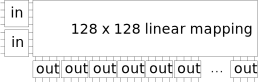
\includegraphics{AES_T1.pdf}}}
    \end{center}
    \caption{Table type I, $8\rightarrow128$ mapping, used for external encoding, taken from \citep{wyseurPhd}}
    \label{fig:aes_t1}
    \end{figure*}
    
    Recall already mentioned T-boxes in section \ref{sec:aes_table} that performs \emph{SubByte} and \emph{AddRoundKey} operations. The \emph{MixColumn} operation 
    is implemented by the matrix multiplication decomposition, these $8\times32$ tables are called $T_y$ boxes. In order to save space
    $T$ and $T_y$ boxes are composed to resulting type II table as illustrates figure \ref{fig:aes_t2}.

    \begin{figure*}[!htb]
    \begin{center}
    \leavevmode
    \centerline{\scalebox{1.0}{\includegraphics{AES_T2.pdf}}}
    \end{center}
    \caption{Table type II, $8\rightarrow32$ mapping, taken from \citep{wyseurPhd}}
    \label{fig:aes_t2}
    \end{figure*}

    Note $32\times32$ mixing bijection added after the \emph{MixColumn} operation to increase diffusion. To cancel this transformation the table 
    type 3 is used as illustrates figure \ref{fig:aes_t3_t4}. Also recall the matrix multiplication decomposition requires addition operation, this is done
    by exclusive-OR (XOR), cascade of table type 4 is used for this purpose. Note that performing XOR by table look-up is rather ineffective, but it is required to 
    protect look-up tables by IO bijections and mixing bijections (to form protected network of look-up tables without revealing true values on 
    table boundaries).
    
    \begin{figure*}[!htb]
    \begin{center}
    \leavevmode
    \centerline{\scalebox{1.0}{\includegraphics{AES_T3_T4.pdf}}}
    \end{center}
    \caption{Table type III and IV, taken from \citep{wyseurPhd}}
    \label{fig:aes_t3_t4}
    \end{figure*}
        

    \paragraph*{Overall scheme.}
    
    Figure \ref{fig:wbaes} illustrates how the round function of whitebox AES implementation for one column looks, using aforementioned tables.
    \begin{figure*}
    \begin{center}
    \leavevmode
    \centerline{\scalebox{1.0}{\includegraphics{WBAES_PQ.pdf}}}
    \end{center}
    \caption{Whitebox AES implementation - round \#2, based on diagram from \citep{Muir_atutorial}}
    \label{fig:wbaes}
    \end{figure*}

    On the diagram in figure \ref{fig:wbaes} are the following mappings:
    \begin{itemize}
    \item MB stands for Mixing Bijection. It is $32 \times 32$ matrix over $\text{GF}(2)$ representing linear transformation over $\text{GF}(2)$. 
    $\text{MB}^{-1}_{\{0,1,2,3\}}$ are then column stripes of corresponding MB inverse matrix (the matrix multiplication decomposition).
    This transformation cancels out within one round. 
    \item L stands also for Mixing Bijection but in this case it is $8 \times 8$ matrix.
    \item Q,P. These are random IO bijections. It holds that $P^{r+1}_{i,j} \circ Q^{r}_{i,j} = id$
    \end{itemize}

    \subsection{Cipher invertibility}\label{sec:cipher_invertibility}
    One of the requirements on the whitebox cipher implementation is usually a~\emph{non-invertibility}. It means that given an encryption part of the cipher 
    with embedded key one should not be able to use it also for decryption and vice versa. This property is especially useful if one wants to use symmetric
    cipher to simulate an asymmetric. But it is important to realize that this goal is difficult to achieve in whitebox context.
    
    As an example take AES whitebox implementation
    Inverting the cipher in blackbox context is rather computationally difficult. Using brute-force one would
    need $2^{128}$ operations to invert the cipher. The whitebox context is in contrast to blackbox advantageous for an attacker. One of the problems here is 
    that ShiftRows operation can be very easily canceled in whitebox context and that attacker can execute only particular round of the cipher. 
    We propose some improvement addressing this problem in section \ref{sec:cipher_invert_improvement}.

    There are 4 columns of state array within one round independent on each other.
    Thus cipher can be easily inverted running the cipher backwards and finding inversion for each column separately, assuming $128\times128$ external mixing bijections
    are $I_{128}$. Thus the task is to find 
    inversion of 32-bit wide function representing one round of the cipher on one column of the state array by running through the space $\text{GF}\left(2^8\right)^4$,
    evaluating the round function and comparing with wanted result.
    
    Computational complexity to invert the cipher
    is $10 \cdot 4 \cdot 2^{32}$ operations \footnote{ $10$ (rounds) $\cdot 4$ (columns) $ \cdot 2^{32}$ (column function input space size)}.
    
    One can also pre-compute tables for inverted cipher, that would occupy $10 \cdot 4 \cdot (2^{32} \cdot 4)\;\text{B} \approx 69\;\text{GB}$.
    We have implemented inversion of WB AES. In non-optimized version it takes 13 hours on my hardware\footnote{For hardware specifications see \ref{appendix:hw_spec}} 
    to invert WB AES with negligible memory requirements.

    \section{The BGE attack}\label{sec:bge_attack}
    The paper \citep{Billet:2004:CWB:2080787.2080809} by Billet~\eal~demonstrated that whitebox AES implementation as described in the previous section is vulnerable
    to an algebraic attack. The attack is named after initials of authors, the BGE attack. It recovers the symmetric key from whitebox AES implementation and
    negligible memory requirements in $2^{30}$ computational steps.
    
    The BGE attack does not analyze look-up tables locally, but instead the whole AES round function is analyzed as a~single look-up table. This has few benefits:
    \begin{itemize}
     \item structure of the round function is fixed and well-known, thus it is easy to model it as an algebraic equation.
     \item $32\times32$ mixing bijections $MB$ is canceled within one round, so they can be neglected.
     \item $8\times8$ mixing bijection $L$ can be easily merged with the IO bijections on round boundary, what simplifies further algebraic analysis. 
    \end{itemize}
    
    Figure \ref{fig:aes_round_bge} illustrates the round function of AES for one column from the BGE attack perspective. Depicted function can 
    be described as a~mapping $\left(x_0, x_1, x_2, x_3\right) \xrightarrow{R^r_j} \left(y_0, y_1, y_2, y_3\right), \; j=0,\dots,3$.   
    
    \begin{figure*}
    \begin{center}
    \leavevmode
    \centerline{\scalebox{1.0}{\includegraphics{BGE_round.pdf}}}
    \end{center}
    \caption{AES round function from the BGE attack perspective, taken from \citep{Billet:2004:CWB:2080787.2080809}}
    \label{fig:aes_round_bge}
    \end{figure*} 

    Since transformation $L$, $L^{-1}$ is performed byte-wise on the state array, it can be composed with corresponding IO bijections, as in equation \ref{eq:ioencoding_abstract_p}.
    \begin{subequations} \label{eq:ioencoding_abstract_q}
    \begin{align}
	Q^{r \; \prime}_{i,j} &= Q^{r}_{i,j} \circ L^{r+1}_{j} \\
	P^{r \; \prime}_{i,j} &= (L^{r}_{j})^{-1} \circ P^{r}_{i,j}
    \end{align}
    \end{subequations}
    The IO bijections are generally non-linear, thus composing it with another linear transformation (L) results again in non-linear bijection. Note that in the BGE
    attack, IO bijections are considered to be general $8\rightarrow8$ bijections, neglecting the fact they are concatenated from 2 $4\rightarrow4$ bijections what allows
    composition with L.
    
    The BGE attack proceeds in three steps:
    \begin{enumerate}
     \item Transform the non-linear IO bijections $Q^{r}_{i,j}$ to unknown $\gf$-affine transformation (i.e. determine non-linear part up to unknown affine part).
     \item Fully determine $Q^{r}_{i,j}$ bijection, using algebraic analysis and known form of the round function.
     \item Obtain round keys from 2 consecutive rounds and recover symmetric key using reversibility of the AES key-schedule.
    \end{enumerate}
    
    \subsection{Recovering non-linear parts}
    This step is particularly interesting because of its universality. It can be applied on different whitebox implementation.
    
    The main goal of this step is to recover non-linear parts of $\left(Q^r_i\right)_{i=0,\dots,3}$. Consider $y_0$ as a~function of $\left(x_0, x_1, x_2, x_3\right)$.
    If $x_1, x_2, x_3$ are fixed as constants $c_1, c_2, c_3$ it is easy to see that the following holds:
    
    \begin{equation} \label{eq:y0}    
    \begin{aligned}
    y_0\left(x_0, c_1, c_2, c_3 \right) &= Q^r_{0,j} \left(\alpha T^r_{0,j}\left(P^r_{0,j}\left(x\right)\right) \oplus \beta_{c_1,c_2,c_3}\right) \\
				        &= Q^r_{0,j} \circ \oplus_{\beta_{c_1,c_2,c_3}} \circ \alpha \cdot T^r_{0,j} \circ P^r_{0,j} \left(x\right)
    \end{aligned}
    \end{equation}
    
    The function $y_0$ from the equation \ref{eq:y0} now takes only $256$ input values, thus the functions $y_0$ and $y_0^{-1}$ 
    can be easily evaluated (as look-up tables). For the rest of the chapter consider constants $c_2, c_3$ fixed, without loss 
    of generality let $c_2=c_3=0$. For the simplification the $r$ superscript is dropped from the 
    equations if it is clear from the context.

    Now assume $c^{\prime}_1 \neq c_1$, also denote $\beta_{0} = \beta_{c_1,c_2,c_3}, \beta_{1} = \beta_{c^{\prime}_1,c_2,c_3}$, it is visible that:
    \begin{subequations}
     \begin{align}
     & y_0\left(x_0, c^{\prime}_1, c_2, c_3 \right) \circ y_0^{-1}\left(x_0, c_1, c_2, c_3 \right) = \nonumber \\
     &=           \left( Q_{0,j}      \circ \oplus_{\beta_1}                         \circ \alpha \cdot T_{0,j}    \circ P_{0,j}     \right) \nonumber
	\circ     \left( P^{-1}_{0,j} \circ \left(\alpha \cdot T_{0,j}\right)^{-1}   \circ \oplus_{\beta_0}        \circ Q^{-1}_{0,j}\right) \nonumber \\
     &= Q_{0,j} \circ \oplus_{\beta_1} \circ \oplus_{\beta_0} \circ Q^{-1}_{0,j}                                                             \nonumber \\
     &= Q_{0,j} \circ \oplus_{\left(\beta_0 \oplus \beta_1\right)} \circ Q^{-1}_{0,j}                                                        \nonumber
     \end{align}
    \end{subequations}

    Thus by fixing $c_1$ and iterating $c^{\prime}_1$ we obtain the set of 256 bijections, represented as look-up tables, 
    of the form $Q_{0,j} \circ \oplus_{\beta} \circ Q^{-1}_{0,j}$, where $\beta$ takes all values from $\gfe$.
    
    \begin{mytheorem}\label{prop:bge1}
     Given a~set of functions $\mathcal{S} = \{Q \circ \oplus_{\beta} \circ Q^{-1}\}_{\beta \in \gfe}$ given by values, 
     where $Q$ is a~permutation of $\gfe$ and the $\oplus_{\beta}$ is the translation by $\beta$ in $\gfe$, one can construct a~particular
     solution $\widetilde{Q}$ such that there exists an affine mapping $A$ so that $\widetilde{Q} = Q \circ A$.
    \end{mytheorem}
    
    For the proof see the original paper \citep{Billet:2004:CWB:2080787.2080809}. In order to recover non-linear part of the IO bijection it is needed to generate
    the set $\mathcal{S}$ (by evaluating $y_0$ functions) and to apply the theorem.
    
    Note that the set $\mathcal{S}$ contains $256$ functions, but only as look-up tables so the $\beta$ is unknown. One easily verifies the set
    $\mathcal{S}$ together with operation of a function composition form a~group. 
    
    Observe there exists isomorphism $\varphi:\; $
    
    \begin{center}
    \begin{tabular}{ r  c c c }
	\multirow{2}{*}{$\varphi \; :$} & $\mathcal{S}$  & $\longrightarrow$ & $\gf^2$ \\
	                                & $Q \circ \oplus_{\beta} \circ Q^{-1} $ & $\longmapsto$ & $\left[ \beta \right]$
	
    \end{tabular}
    \end{center}
    
    Since we don't know the values $\beta$ for the functions in $\mathcal{S}$ the $\varphi$ cannot be constructed directly, however it is possible to 
    recover $\varphi$ up to unknown linear transformation $L$ i.e. $\psi = L^{-1} \circ \varphi$. Without going into details, the 
    $\psi$ is determined by finding base functions $f_1,\dots,f_8$ that spans the whole $\mathcal{S}$ under composition. Mapping $\psi$ is then constructed by assigning
    standard basis vectors $e_1,\dots,e_8 \in \gf^8$ to these functions.
    
    It is then possible to obtain $\widetilde{Q}$ by using the mapping $\psi$ from the theorem \ref{prop:bge1} according to the following formula:
    \begin{equation}\label{eq:Qtilde}
     \widetilde{Q}\left(\psi\left(g\right)\right) = g\left(0\right),\; g \in \mathcal{S}
    \end{equation}
    
    Note that the value $g\left(0\right)$ is known, the function was evaluated during $\psi$ construction. The term $\psi\left(g\right)$ is also easy to
    evaluate, since we have constructed mapping $\psi$. Thus in order to recover $\widetilde{Q}$ as a~look-up table we just run over the set $\widetilde{Q}$
    and compute the values of mapping $\widetilde{Q}$ according to the equation \ref{eq:Qtilde}.
    
    \subsection{Recovering the symmetric key}
    As the rest of the BGE attack is very AES and implementation specific it is not covered in detail. In this phase, we are still in situation as
    depicted in figure \ref{fig:aes_round_bge} with a difference $\left(Q^r_i\right)_{i=0,\dots,3}$ and $\left(P^{r+1}_i\right)_{i=0,\dots,3}$
    are affine, still matching, bijections. This fact makes further algebraic analysis of round function possible.
    
    Consider following useful proposition:
    \begin{myprop}\label{prop:bge_prop1}
     For any pair $\left(y_i, y_j\right)$ exists a unique linear mapping $L$ and a unique constant $c$ such that:
     \begin{equation}
	\forall x_0 \in \gfe:\; y_i\left(x_0, 0, 0, 0\right) = L \left(y_j \left(x_0, 0, 0, 0 \right) \right) \oplus c
     \end{equation}
    \end{myprop}
    
    By using \ref{prop:bge_prop1} one can obtain the linear parts of $Q_1, Q_2, Q_3$ from the knowledge of the $Q_0$ linear part in $2^{16}$ steps by simple
    running over $c$ and testing the resulting mapping for linearity in $2^8$ steps. Thus the rest of the attack focuses on $Q_0$ determination.
    
    First of all, the linear part of $Q_0$ up to $\left[\gamma\right], \gamma \in \gfe \setminus \{0\}$ is determined, where $\left[\gamma\right]$ denotes the
    matrix in $\gf$ corresponding to multiplication by $\gamma$ in $\gfe$, for more details see appendix \ref{appendix:mult_matrix}.
    
    Then $\gamma$ and constant part $q_0$ of $Q_0$ are determined. During this steps, the public knowledge of S-boxes and MixColumn matrix coefficients is used.
    
    With completely determined $Q_0$ the round keys are extracted.
    The attack ends using the fact the key-schedule of AES is reversible, so from two consecutive round keys one can derive original symmetric key.
    
\chapter{WBCAR AES using dual ciphers}\label{sec:wb_dual_aes_sec}
    WBCAR stands for whitebox context attack resistant, meaning cipher implementation should resist attacks like key-extraction, cipher inversion
    and others against attacker in whitebox context.
    
    In this chapter I describe whitebox scheme proposed in \citep{Karroumi:2010:PWA:2041036.2041060} that make use of AES dual ciphers. It is supposed 
    that using dual AES, different in each round, will increase security of whitebox implementation of the cipher. Paper says that this modification
    results in raising BGE attack \citep{Billet:2004:CWB:2080787.2080809} complexity to $2^{91}$ computational steps, making it unfeasible to perform it in practice. It is shown in section
    \ref{sec:attacking_dual_aes} that this assumption is false due to existence of an attack we performed.
    
    
    \section{Scheme}

    In the original paper \citep{Karroumi:2010:PWA:2041036.2041060} the explanation how to obtain dual AES ciphers and how to construct mapping from one 
    to another is not given. This is
    important part since it plays crucial role in a~proof that this scheme is vulnerable. At first is described generalization of the AES and how to construct
    mappings between them. 

	\subsection{Ciphers duality}
	This section introduces notion of dual ciphers used in this chapter. Dual ciphers has interesting properties and are used in construction
	of the scheme that is described by this chapter. Consider the following definition.
	
	\begin{mydef}\label{def:dual_cipher}
	Two ciphers $E$ and $E'$ are called Dual Ciphers, if they are
	isomorphic, i.e., if there exist invertible transformations $f$, $g$ and $h$ such
	that

	\begin{equation} 
	\forall p, k: E_k(p) = f^{-1}\left(E'_{g(k)}(h(p))\right)
	\end{equation}
	where $p$ is the plaintext, and $k$ is the secret key.
	\end{mydef}

	\subsection{Generic AES}
	It is possible to generalize AES by changing its irreducible polynomial and generator to obtain generic form of AES.

	Generic AES can be represented as a~$\{R(x), \beta \}$, where $R(x) \in \left(\mathbb{Z}/p\mathbb{Z}\right)[x]$ is 
	irreducible polynomial of degree 8, $\beta \in \gfe$ is a~generator of the field $\gfe$.

	Default AES (as in NIST standard) in this notation is represented as $\{\{11B\}_x, \{03\}_x\}$. Polynomial is expressed
	in hexadecimal notation, each bit corresponds to polynomial coefficient, LSB corresponds to constant term.\\
	Thus $0x11B_{16} = 1 \; 0001 \; 1011_{2} \; \Rightarrow \{11B\}_x \sim x^8+x^4+x^3+x+1$.

	It is known that there are $30$ irreducible polynomials over $\gfe$. For each of them there are $8$ possible
	generators that can be used to generate field and to preserve duality mentioned in the next section.

	\subsection{Generic AES duality}
	Let's assume we have some arbitrary generic AES $\{R(x), \beta \}$. 

	All elements of the field $\gfe = \{01, 02, \dots, FF\}$
	can be expressed in terms of the generator $\beta$, $\gfe = \{\beta^i \; | \; i \in [0,254]\} = \{\beta^0, \beta^1, \dots, \beta^{254}\}$.

	We can then construct $8 \times 8$ matrix $\Delta = \begin{bmatrix} \beta^0 & \beta^{25} & \beta^{50} & \beta^{75} & \beta^{100} & \beta^{125} & \beta^{150} & \beta^{175}  \end{bmatrix}$ where 
	$\beta^i \in \gfe \cong \text{GF}(2)^8$ is a~column vector. Then $\Delta$ is a~base change matrix:
	\begin{subequations}
	\begin{align}
	    \Delta &: \{\{11B\}_x, \{03\}_x\}  \longrightarrow \{R(x), \beta \} \\
	    \Delta^{-1} &: \{R(x), \beta \}  \longrightarrow \{\{11B\}_x, \{03\}_x\}
	\end{align}
	\end{subequations}

	For default AES $\{\{11B\}_x, \{03\}_x\}$ holds
	\begin{align*}
	    \Delta &= \begin{bmatrix} 03^0 & 03^{25} & 03^{50} & 03^{75} & 03^{100} & 03^{125} & 03^{150} & 03^{175}  \end{bmatrix} \\
	           &= \begin{bmatrix} 01 & 02 & 04 & 08 & 16 & 32 & 64 & 128 \end{bmatrix} \\
		   &= I_8
	\end{align*}
	as expected.

	From this it is clear that following duality holds: $E \sim \{\{11B\}_x, \{03\}_x\}, \; E' \sim \{R(x), \beta \}$ then:
	\begin{equation} 
	\forall p, k: E_k(p) = \Delta^{-1}\left(E'_{\Delta(k)}(\Delta(p))\right)
	\end{equation}

	\subsection{Constructing Dual AES}
	We can construct arbitrary dual AES from default AES. Recall there are 4 operations used in single AES round: \emph{ShiftRows}, \emph{AddRoundKey}, \emph{SubByte}, \emph{MixColumn}.

	\paragraph*{Default AES}
	\emph{ShiftRows}, \emph{AddRoundKey} functions are quite simple and remain same after AES generalization. \emph{SubByte}, \emph{MixColumn} are affected by 
	generalization, for proper understanding of construction generic AES, description follows.

	\subparagraph*{SubByte}\label{sec:aes_subbyte}
	\begin{equation}
	\begin{aligned}
	S: \gfe         & \longrightarrow  \gfe\\
	x               & \longmapsto A \times x^{-1} \oplus c
	\end{aligned}
	\end{equation}
	where $x^{-1}$ is element inverse in $\gfe$, A is $8 \times 8$ matrix over $\text{GF}(2)$, c is column vector $\text{GF}(2)^8$. A, c are constants defined in NIST standard.

	Equation for affine transformation used in S-box:
	\begin{align}
		\begin{bmatrix}
		    y_0\\
		    y_1\\
		    y_2\\
		    y_3\\
		    y_4\\
		    y_5\\
		    y_6\\
		    y_7\\
		\end{bmatrix}
		    =
		\begin{bmatrix}
		    1 & 0 & 0 & 0 & 1 & 1 & 1 & 1 \\
		    1 & 1 & 0 & 0 & 0 & 1 & 1 & 1 \\
		    1 & 1 & 1 & 0 & 0 & 0 & 1 & 1 \\
		    1 & 1 & 1 & 1 & 0 & 0 & 0 & 1 \\
		    1 & 1 & 1 & 1 & 1 & 0 & 0 & 0 \\
		    0 & 1 & 1 & 1 & 1 & 1 & 0 & 0 \\
		    0 & 0 & 1 & 1 & 1 & 1 & 1 & 0 \\
		    0 & 0 & 0 & 0 & 1 & 1 & 1 & 1 \\
		\end{bmatrix}
		\begin{bmatrix}
		    x_0\\
		    x_1\\
		    x_2\\
		    x_3\\
		    x_4\\
		    x_5\\
		    x_6\\
		    x_7\\
		\end{bmatrix}
		    +
		\begin{bmatrix}
		    1\\
		    1\\
		    0\\
		    0\\
		    0\\
		    1\\
		    1\\
		    0\\
		\end{bmatrix}
	    \end{align}
	where $x_i, y_i \in \text{GF}(2)$.

	\subparagraph*{MixColumn}
	    \begin{itemize}
	    \item columns considered as polynomials over $\gfe$
	    \item $p(x) \cdot c(x) \imod{x^4+1}$\\
	    where $c(x)$ is fixed polynomial $c(x) = 03x^3+01x^2 + 01x + 02$
	    \end{itemize}
	    \begin{align}
		\begin{bmatrix}
		    y_0\\
		    y_1\\
		    y_2\\
		    y_3\\
		\end{bmatrix}
		    =	
		\begin{bmatrix}
		    02 & 03 & 01 & 01\\
		    01 & 02 & 03 & 01\\
		    01 & 01 & 02 & 03\\
		    03 & 01 & 01 & 02\\
		\end{bmatrix}
		\begin{bmatrix}
		    x_0\\
		    x_1\\
		    x_2\\
		    x_3\\
		\end{bmatrix}
	    \end{align}
	where $x_i, y_i \in \gfe$.
	
	\paragraph*{Generic AES}
	In the generic AES, the operations \emph{ShiftRows}, \emph{AddRoundKey} work same as in default AES, they are not affected by base change operation.

	\subparagraph*{SubByte}\label{sec:aes_generic_subbyte}
	\begin{equation}
	\begin{aligned}
	S_{dual}: \gfe           & \longrightarrow  \gfe\\
	x                        & \longmapsto \Delta \times A \times \Delta^{-1} \left( x^{-1} \right) \oplus \Delta \left(c\right)
	\end{aligned}
	\end{equation}

	\subparagraph*{MixColumn}
	MixColumn matrix coefficients are expressed in terms of generator $\beta = 03$.
	\[
	\begin{bmatrix}
		    \beta^{25} & \beta^{1} & \beta^{0} & \beta^{0}\\
		    \beta^{0} & \beta^{25} & \beta^{1} & \beta^{0}\\
		    \beta^{0} & \beta^{0} & \beta^{25} & \beta^{1}\\
		    \beta^{1} & \beta^{0} & \beta^{0} & \beta^{25}\\
	\end{bmatrix}
	\]

	\paragraph*{Round function - default AES}
	We consider whole AES round as a~single function $R$ of a~state array. Let's define
	\[
	\begin{bmatrix} 
	    x_{0,0} & x_{0,1} & x_{0,2} & x_{0,3}\\
	    x_{1,0} & x_{1,1} & x_{1,2} & x_{1,3}\\
	    x_{2,0} & x_{2,1} & x_{2,2} & x_{2,3}\\
	    x_{3,0} & x_{3,1} & x_{3,2} & x_{3,3}\\
	\end{bmatrix} 
	\overset{R}{\longrightarrow}
	\begin{bmatrix} 
	    y_{0,0} & y_{0,1} & y_{0,2} & y_{0,3}\\
	    y_{1,0} & y_{1,1} & y_{1,2} & y_{1,3}\\
	    y_{2,0} & y_{2,1} & y_{2,2} & y_{2,3}\\
	    y_{3,0} & y_{3,1} & y_{3,2} & y_{3,3}\\
	\end{bmatrix} 
	\]

	From this we define $y_{i,j}$ as a~function with 4 arguments from $\gfe$:
	\begin{equation}
	y_{i,j}\left(x_{i,0}, x_{i,1}, x_{i,2}, x_{i,3}\right) = \bigoplus^3_{l=0} \alpha_{l,j} \cdot S(x_{i,l} \oplus k_{i,l})
	\end{equation}
	where $\alpha_{k,j}$ is MixColumn matrix coefficient in $k$-th row and $j$-th column. We are abstracting here \emph{ShiftRows} operation, it won't be needed for our further argumentation.
	To make it clear here are equations for the first column of state array:

	{\footnotesize
	\begin{subequations}
	\begin{align}
	y_{0,0}\left(x_{0,0}, x_{1,0}, x_{2,0}, x_{3,0}\right) &= 02 \cdot T_{0,0}(x_{0,0}) \oplus 03 \cdot T_{1,0}(x_{1,0})\oplus 01 \cdot T_{2,0}(x_{2,0})\oplus 01 \cdot T_{3,0}(x_{3,0})\\
	y_{1,0}\left(x_{0,0}, x_{1,0}, x_{2,0}, x_{3,0}\right) &= 01 \cdot T_{0,0}(x_{0,0}) \oplus 02 \cdot T_{1,0}(x_{1,0})\oplus 03 \cdot T_{2,0}(x_{2,0})\oplus 01 \cdot T_{3,0}(x_{3,0})\\
	y_{2,0}\left(x_{0,0}, x_{1,0}, x_{2,0}, x_{3,0}\right) &= 01 \cdot T_{0,0}(x_{0,0}) \oplus 01 \cdot T_{1,0}(x_{1,0})\oplus 02 \cdot T_{2,0}(x_{2,0})\oplus 03 \cdot T_{3,0}(x_{3,0})\\
	y_{3,0}\left(x_{0,0}, x_{1,0}, x_{2,0}, x_{3,0}\right) &= 03 \cdot T_{0,0}(x_{0,0}) \oplus 01 \cdot T_{1,0}(x_{1,0})\oplus 01 \cdot T_{2,0}(x_{2,0})\oplus 02 \cdot T_{3,0}(x_{3,0})
	\end{align}
	\end{subequations}}
	where $T_{i,j}(x) = S\left(x \oplus k_{i,j}\right)$.

	\paragraph*{Round function - generic AES}
	Using aforementioned generic form of \emph{SubByte} and \emph{MixColumn} functions we can define round function also for generic AES in the same way, using base change transformation.
	From this we define $y_{i,j}$ as a~function with 4 arguments from $\gfe$:
	\begin{equation}
	y_{i,j}\left(x_{i,0}, x_{i,1}, x_{i,2}, x_{i,3}\right) = \bigoplus^3_{l=0} \Delta(\alpha_{l,j}) \cdot \left( \Delta \times A \times \Delta^{-1} \left( \left(x_{i,l} \oplus \Delta\left(k_{i,l}\right) \right)^{-1} \right) \oplus \Delta \left(c\right) \right)
	\end{equation}

	\subsection{Whitebox Dual AES}\label{sec:wb_dual_aes}
	The paper describing AES whitebox implementation with use of dual AES \citep{Karroumi:2010:PWA:2041036.2041060}, claimed that this implementation should be harder (in terms of time complexity)
	to break using the BGE attack on whitebox AES. On the figure \ref{fig:wbaesdual} is scheme for one round, one column of state array, whitebox dual AES implementation for round 2.
	According to the original paper, in each
	column is used different generic AES. This implementation is compatible with default AES, so after computing in dual AES we have to transform the result to default AES
	with base change transformation $\Delta$.\\

	% scheme for one round of WB Dual AES
	\begin{figure*}
	\begin{center}
	\leavevmode
	\centerline{\scalebox{0.9}{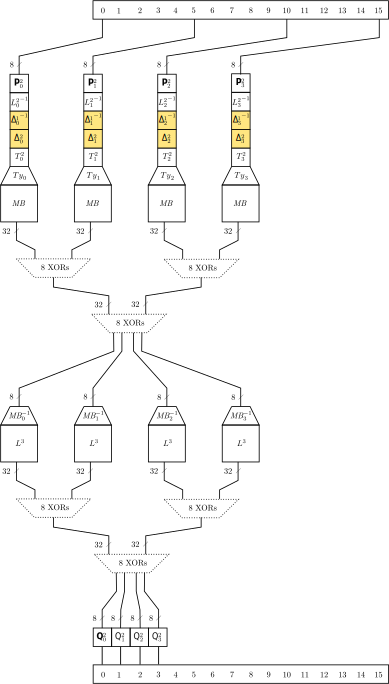
\includegraphics{WBAES_PQ_DUAL.pdf}}}
	\end{center}
	\caption{Whitebox Dual AES implementation - round \#2, based on diagram from \citep{Muir_atutorial}}
	\label{fig:wbaesdual}
	\end{figure*}
	
	By changing irreducible polynomial and generator we obtain $30 \cdot 8 = 240$ different generic AES ciphers. The bigger is set of possible ciphers to use, the harder is
	for attacker to break the dual scheme, since he has to try all possible combinations, according to \citep{Karroumi:2010:PWA:2041036.2041060}. But in 
	\citep{Karroumi:2010:PWA:2041036.2041060} is assumed there are $61200$ different generic AES ciphers but it is not said how they are constructed and how 
	such construction influences whitebox implementation.
	
	In order to generate $61200$ different AES representations it is needed to study AES S-Box affine self-equivalences \citep{Biryukov:2003:TCL:1766171.1766175}. 
		
	\begin{mydef}
	$n \times n$-bit mapping $S$ is affine self-equivalent if there exist $n \times n$ affine relations $A_1,\;A_2$ such that: 
	\begin{equation}\label{eq:selfeq}
	A_2 \circ S \circ A_1 = S 
	\end{equation}
	\end{mydef}
	
	In \citep{Biryukov:2003:TCL:1766171.1766175} are published effective algorithms for finding linear and affine equivalences for permutations (S-boxes). I have implemented
	them \footnote{path: implementation/LinearAffineEq.\{h,cpp\}} to verify number of self-equivalences for AES S-Boxes for encryption and decryption algorithm. 
	This algorithm can be further used to study modified S-boxed or basic building blocks of the cipher (see chapter \ref{sec:twofish_sbox}) for equivalences, what can lead
	to revealing potential weaknesses.
	
	Algorithm found $2040$ affine self-equivalences, together with $30$ possible irreducible polynomials there are $61200$ dual ciphers.
	Biryukov \emph{et~al.} derived general expressions for $A_1,\;A_2$:
	\begin{subequations}
	\begin{align}
	    A_1(x) &= \left[a\right] \cdot Q^i \cdot x\\
	    A_2(x) &= A\left( Q^{-i} \cdot \left[a\right] \cdot A^{-1}\left(x\right) \right)
	\end{align}
	\end{subequations}
	
	Where
	\begin{itemize}[leftmargin=5em]
	 \item[{$A$}] is fixed affine mapping from AES S-box definition (see section \ref{sec:aes_subbyte}), $A^{-1}$ it's inverse.
	 \item[{$[a]$}] denotes $8 \times 8$ matrix with coefficients from $\gf$ representing \emph{multiplication} by $a \in \gfe \setminus \{0\}$ in $\gfe$. 
	    From the fact $\gf^8 \simeq \gfe$ (all finite fields with same number of elements are isomorphic), multiplication is
	    linear transformation in $\gfe$, it can be expressed in matrix form. Refer to \ref{appendix:mult_matrix} to see how to construct such matrix.
	 \item[{$Q$}] denotes $8 \times 8$ matrix with coefficients from $\gf$ representing \emph{squaring} in $\gfe$. Squaring is \emph{linear} operation
	    in $\gfe$ so it is possible to represent it as a~matrix. Refer to \ref{appendix:sqr_matrix} for construction and proof. Note that 
	    $Q^8 = I \Rightarrow Q^{-i} = Q^{8-i}$. Thus there are 8 different powers of Q, $Q^{i}, \; i \in [0,7]$.
	\end{itemize}
	
	It is visible that with general expressions we can obtain $8 \cdot 255 = 2040$ different 
	$A_1,\;A_2$ relations\footnote{by running through possible values for $a,i$ } confirming output of the algorithm. 
	
	Observe that by inserting $A_1,\;A_2$ before and after S-Box the cipher is not affected. Note that $A_1$ is linear, this can be used to 
	push input mapping $A_1$ through the mixing layer and combine it with $A_2$ from previous round, then we obtain $2040$ different AES 
	tables evaluating the same function. Note that they are not dual according to definition \ref{def:dual_cipher}, it is just different 
	table implementation of AES, thus $\Delta = I$. This is potential flaw of whitebox scheme using dual ciphers, since it does not increase
	security against known attacks at all. This construction is neglected in the original paper \citep{Karroumi:2010:PWA:2041036.2041060}.
	
	Layers of mixing bijections (L, MB) cancel between rounds so they can be neglected in pushing $A_1$ to previous round. 
	%At first consider that in previous and current round we have standard AES, further it will be extended for generic case. 
	Recall $A_2\left(S\left(A_1\left(x\right)\right)\right) = S(x)$. Input to S-box is output of previous round, so apply $A_1$ on previous round.
	It is shown only for one column (equation \ref{eq:a1_application}), others are analogical. It is easy to verify that 
	$\left[a\right] \cdot Q^i \cdot \left[c\right] = \left[c^{2^{i}}\right] \cdot \left[c\right] \cdot Q^i$. 
	Redefine $T_r(x) = A_2^r(S(x \oplus k))$ to take affine relations into account, where $k$ is particular round key byte. Then we can write:

	% A_1^{r+1, i}(x) &= [l] \cdot Q^k (x)
	
	{%\footnotesize
	\begin{subequations}\label{eq:a1_application}
	\begin{align}
	       A_1^{r+1} \cdot &\begin{bmatrix}           02 \cdot T_r(x)        &           01 \cdot T_r(x)        &           01 \cdot T_r(x)        &           03 \cdot T_r(x)        \end{bmatrix}^T \label{eq:a1_application_1} \\
	    =                  &\begin{bmatrix} A_1^{r+1}(02 \cdot T_r(x))       & A_1^{r+1}(01 \cdot T_r(x))       & A_1^{r+1}(01 \cdot T_r(x))       & A_1^{r+1}(03 \cdot T_r(x))       \end{bmatrix}^T \nonumber\\
	    =                  &\begin{bmatrix} 02^{2^i} \cdot A_1^{r+1}(T_r(x)) & 01^{2^i} \cdot A_1^{r+1}(T_r(x)) & 01^{2^i} \cdot A_1^{r+1}(T_r(x)) & 03^{2^i} \cdot A_1^{r+1}(T_r(x)) \end{bmatrix}^T \nonumber\\
	    =                  &\begin{bmatrix} 02^{2^i} \cdot A_1^{r+1}(T_r(x)) & 01 \cdot A_1^{r+1}(T_r(x))       & 01 \cdot A_1^{r+1}(T_r(x))       & 03^{2^i} \cdot A_1^{r+1}(T_r(x)) \end{bmatrix}^T
	\end{align}
	\end{subequations}}
	
	This gives us different tables for AES round function when using different $A_1,\;A_2$ relations. Note that table of type 2 with $A_1$ pushed from next round 
	is still the same, no matter which form of equation \ref{eq:a1_application} is used, due to linearity of $A_1$. 
	For simplicity in further proofs and description we can assume form \ref{eq:a1_application_1}.

    \section{Attacking Dual AES scheme}\label{sec:attacking_dual_aes}
	According to \citep{Karroumi:2010:PWA:2041036.2041060} whitebox scheme using Dual AES is considered to be more difficult to crack with BGE attack and thus it is consider
	safer than original scheme proposed in \citep{Chow02white-boxcryptography}. But we show that it is not true. This result was not published yet.
	
	\begin{myprop}
	Whitebox Dual AES scheme can be broken with the BGE attack with the same time complexity as Whitebox AES scheme.
	\end{myprop}

	\begin{proof}
	Let's define round function for whitebox AES and for whitebox dual AES and compare it. 
	Note that MB mixing bijections are left out since their effect is canceled within one round. If we also assume use of $A_1, \; A_2$ affine relations,
	they can be merged together with L mixing bijection to input/output encodings. Thus for simplicity $A_1, \; A_2$ is omitted from the proof (it is clearly visible 
	it does not increase resistance against BGE attack - input/output encodings are fully determined in the attack).

	\paragraph*{Round function - whitebox AES.}
	There are additional $Q' ,P' $ functions, input and output bijections, for details see \citep{Chow02white-boxcryptography} \citep{Billet:2004:CWB:2080787.2080809}.
	\begin{subequations}
	\begin{align} 
	y_{i,j}\left(x_{i,0}, x_{i,1}, x_{i,2}, x_{i,3}\right)  &= Q^{r \; \prime}_{i,j}\left( \bigoplus^3_{l=0} \alpha_{l,j} \cdot S \left(P^{r \; \prime}_{i,l}\left(x_{i,l}\right) \right) \right) \\
								&= Q^{r \; \prime}_{i,j}\left( \bigoplus^3_{l=0} \alpha_{l,j} \cdot \left( A \left( \left(P^{r \; \prime}_{i,l}\left(x_{i,l}\right) \oplus k_{i,l} \right)^{-1} \right) \oplus c \right) \right) \\
								&= Q^{r \; \prime}_{i,j} \circ R_{i,j}\left(x_{i,0}, x_{i,1}, x_{i,2}, x_{i,3}\right) \label{eq:whitebox_aes_roud}
	\end{align}
	\end{subequations}

	\paragraph*{Round function - whitebox dual AES.}
	For simplicity define:
	\begin{equation}
	    P^{r \; \prime\prime}_{i,j} = \left(\Delta^{r-1}\right)^{-1} \circ P^{r \; \prime}_{i,j} = \left(\Delta^{r-1}\right)^{-1} \circ (L^{r}_{j})^{-1} \circ P^{r}_{i,j} \label{eq:ioencoding_abstract_p}
	\end{equation}
	Also we have to distinguish in which dual AES is element encoded, so define $x^{\Delta}$ as a~element of the dual AES which base change matrix is $\Delta$ from standard AES field. 
	The same holds for inversion operation $^{-1}$. Denote $^{-1^{\Delta}}$ inversion in field of dual AES which has base change matrix $\Delta$.
	
	For simplicity assume that $\Delta = \Delta^r$ for round $r$ if it is obvious from context and is not defined otherwise.
	According to figure \ref{fig:wbaesdual} the equation for one round is:
	\begin{subequations} \label{eq:wb_dual_aes_r_proof}
	\begin{align} 
	& y_{i,j}\left(x_{i,0}, x_{i,1}, x_{i,2}, x_{i,3}\right) = \nonumber \\
	&= Q^{r \; \prime}_{i,j}              \left( \bigoplus^3_{l=0} \Delta(\alpha_{l,j}) \cdot \left( \Delta \times A \times \Delta^{-1} \left(               \left(\Delta \circ P^{r \; \prime\prime}_{i,l}\left(x_{i,l}\right) \oplus \Delta\left(k_{i,l}\right) \right)^{-1^{\Delta}\; \gfe} \right) \oplus \Delta \left(c\right) \right) \right) \nonumber \\ 
	&= Q^{r \; \prime}_{i,j} \circ \Delta \left( \bigoplus^3_{l=0}        \alpha_{l,j}  \cdot \left(               A \times \Delta^{-1} \left(               \left(\Delta \circ P^{r \; \prime\prime}_{i,l}\left(x_{i,l}\right) \oplus \Delta\left(k_{i,l}\right) \right)^{-1^{\Delta}\; \gfe} \right) \oplus              c        \right) \right) \nonumber \\ 
	&= Q^{r \; \prime}_{i,j} \circ \Delta \left( \bigoplus^3_{l=0}        \alpha_{l,j}  \cdot \left(               A \times \Delta^{-1} \left( \left( \Delta \left(             P^{r \; \prime\prime}_{i,l}\left(x_{i,l}\right) \oplus             k_{i,l}\right) \right)^{-1^{\Delta}\; \gfe} \right) \oplus              c        \right) \right) \label{eq:wb_dual_aes_r_proof1} \\ 
	&= Q^{r \; \prime}_{i,j} \circ \Delta \left( \bigoplus^3_{l=0}        \alpha_{l,j}  \cdot \left(               A \times \Delta^{-1} \left( \Delta        \left(             P^{r \; \prime\prime}_{i,l}\left(x_{i,l}\right) \oplus             k_{i,l}        \right)^{-1\; \gfe} \right)          \oplus              c        \right) \right) \label{eq:wb_dual_aes_r_proof2} \\
	&= Q^{r \; \prime}_{i,j} \circ \Delta \left( \bigoplus^3_{l=0}        \alpha_{l,j}  \cdot \left(               A \times             \left(               \left(             P^{r \; \prime\prime}_{i,l}\left(x_{i,l}\right) \oplus             k_{i,l}        \right)^{-1\; \gfe} \right)          \oplus              c        \right) \right) \nonumber\\
	&= Q^{r \; \prime}_{i,j} \circ \Delta \left( \bigoplus^3_{l=0}        \alpha_{l,j}  \cdot \left(               A \times             \left(               \left(             P^{r \; \prime\prime}_{i,l}\left(x_{i,l}\right) \oplus             k_{i,l}        \right)^{-1\; \gfe} \right)          \oplus              c        \right) \right) \nonumber\\
	&= Q^{r \; \prime}_{i,j} \circ \Delta \circ R_{i,j}^{\prime}\left(x_{i,0}, x_{i,1}, x_{i,2}, x_{i,3}\right) \label{eq:wb_dual_aes_r_prooffinal}
	\end{align}
	\end{subequations}

	Now it is easy to see whitebox dual AES correctness, moreover it is visible that the same attack breaking whitebox AES breaks whitebox dual AES scheme. 

	Transformation from \ref{eq:wb_dual_aes_r_proof1} to \ref{eq:wb_dual_aes_r_proof2} is possible due to base change matrix properties and fields we are computing in.
	\begin{align}
	    \forall x,y \in \gfe \; : \; y = x^{-1} \Rightarrow  \Delta y = \left( \Delta x \right)^{-1^{\Delta}}
	\end{align}
	Note that element inversion $\gfe$ has changed from one field to another.

	Now if we compare equations \ref{eq:whitebox_aes_roud} and \ref{eq:wb_dual_aes_r_prooffinal}, they are very similar, 
	the only difference here is the application of base change matrix $\Delta$.

	Here we can do the similar thing we did in equations \ref{eq:ioencoding_abstract_q}, \ref{eq:ioencoding_abstract_p} where we composed
	two transformations, non-linear and linear to non-linear transformation, with equation \ref{eq:wb_dual_aes_r_prooffinal}. 

	We can thus define:
	\begin{subequations}
	\begin{align}
	    Q^{r \; \prime\prime}_{i,j} &= Q^{r \; \prime}_{i,j} = Q^{r}_{i,j} \circ \Delta = Q^{r}_{i,j} \circ L^{r+1}_{j} \circ \Delta \\
	    y_{i,j}\left(x_{i,0}, x_{i,1}, x_{i,2}, x_{i,3}\right) &= Q^{r \; \prime}_{i,j}       \circ \Delta \circ R_{i,j}\left(x_{i,0}, x_{i,1}, x_{i,2}, x_{i,3}\right) \\
	    y_{i,j}\left(x_{i,0}, x_{i,1}, x_{i,2}, x_{i,3}\right) &= Q^{r \; \prime\prime}_{i,j} \circ R_{i,j}\left(x_{i,0}, x_{i,1}, x_{i,2}, x_{i,3}\right) \label{eq:whitebox_dual_aes_round}
	\end{align}
	\end{subequations}

	Now it is evident that equations for whitebox AES \ref{eq:whitebox_aes_roud} and \ref{eq:whitebox_dual_aes_round} are the same, the only difference is only in non-linear 
	transformations $Q$, but it is important they are both non-linear. 

	Conclusion is if attack can break whitebox AES scheme with round function \ref{eq:whitebox_aes_roud} it can also break whitebox dual AES scheme. During the attack is transformation $Q$ 
	fully determined, we verified that if Dual AES scheme is used, transformation $Q$ is the exact form as described above.
	\end{proof}

    \section{Implementation of the cipher}
%    [TODO] Cipher implementation description, generalization of oorschot design. Mixing bijections.
    As the part of the assignment of this thesis was to implement 2--3 whitebox AES schemes, together with cryptanalysis, if is available. 
    The scheme using dual AES was chosen to be implemented, since in the time of making this decision there was no published cryptanalysis
    of this scheme and it had interesting and easy construction. The fact it is generalization of the original whitebox AES scheme
    published by Chow~\eal~is additional benefit what simplifies the implementation.
    
    \subsection{NTL library}
    Recall AES cipher uses finite fields algebra extensively, namely in $\gf$ and $\gfe$. For this reason the library
    NTL\footnote{NTL is a high-performance, portable C++ library providing data structures and algorithms for manipulating signed, arbitrary length integers, 
	and for vectors, matrices, and polynomials over the integers and over finite fields. \url{http://www.shoup.net/ntl/}} was selected
    as a cornerstone of this implementation. It enables both an effective computation in the finite fields and to write simple, understandable and easy-to-read
    source code. 
    
    Besides NTL there was no need to use any other math library.
    
    \subsection{Generic AES}
    In order to be able to implement whitebox AES implementation, it was necessary to implement the basic building blocks of the AES as described in
    previous chapters (such as S-boxes, MixColumn, etc...), using the NTL library. It was preferred to implement it from the scratch, according to the specification,
    rather than taking existing implementations. The emphasis was put on a simple and extendable source code, rather than optimized and difficult to understand. 
    The another reason was the fact that AES implementations work with fixed finite field (as generated by irreducible polynomial and a generator - according 
    to the AES specifications) so the algebraic nature of the operations was not clear from the code anymore, because of various optimizations. Due to the fact
    dual AES scheme uses generalized AES, it was needed to generate such AES instances with changed irreducible polynomial and the generator. 
    
    The output from the key-schedule (generated by generic AES) was also required by whitebox implementation.
    
    \subsection{Mixing Bijections}
    As described in section \ref{sec:whitebox_aes_scheme_chow} the mixing bijection matrices has to have special form in order to provide sufficient 
    level of protection. The algorithm described by Zhou~\eal in \citep{journals/iacr/XiaoZ02} to generate matrices with desired properties was implemented.
    
    This part of the implementation is independent on whitebox context and thus can be used separately, to generate matrices with good diffusion properties.
    
    In order to implement mentioned algorithm it was necessary to extend the NTL library. Namely it was needed to generate such matrices $P, Q$ for matrix $A$
    so that the equation \ref{eq:normal_matrix_form} holds. The Gauss-Jordan elimination was modified to generate these matrices\footnote{Matrix $P$ corresponds to multiplication of 
    elementary row matrices that transforms matrix A to row-echelon form. The matrix $Q$ corresponds to multiplication by column elementary matrices that
    reorder the columns in a way the equation \ref{eq:normal_matrix_form} holds.}

    \begin{equation}\label{eq:normal_matrix_form}
	P \cdot A \cdot Q = 
	\begin{bmatrix}
	    1      & \cdots & 0      & 0      & \cdots & \cdots & 0      \\
	    \vdots & \ddots & \vdots & \vdots &        &        & \vdots \\ 
	    0      & \cdots & 1      & 0      & \cdots & \cdots & 0      \\
	    0      & \cdots & 0      & 0      & \cdots & \cdots & 0      \\
	    \vdots & \ddots & \vdots & \vdots &        &        & \vdots \\ 
	    0      & \cdots & 0      & 0      & \cdots & \cdots & 0      
	\end{bmatrix}
    \end{equation}
    
    It is also needed to generate a random linear transformation in the algorithm. The number of all possible $p \times p$ matrices 
    in $\mathbb{F}_q$ is $q^{p\cdot p}$, while the number of all possible non-singular (invertible) matrices is $\prod_{i=0}^{p-1}(q^p - q^i)$.
    In our case $q=2, \; \mathbb{F}_q \equiv \gf$. The table \ref{tbl:random_matrix_nonsingular_probab} shows the probability of randomly generated matrix of particular 
    dimension being non-singluar. For our parameters the value converges around $0.2888$ so it is enough to generate a random matrix
    and test whether it is invertible. Within 4 iterations the non-singular matrix is found with sufficient high probability.

    The rest of the algorithm for construction mixing bijections follows the paper by Zhou~\eal.
    
    \begin{table}[!htb]
    \begin{center}
    \begin{tabular}{ | c | r | }
	\hline
	dimension     & probability    \\ \hline \hline
	$2\times2$    & $0.375$        \\ \hline
	$4\times4$    & $ 0.30762$     \\ \hline
	$8\times8$    & $ 0.28992$     \\ \hline
	$16\times16$  & $ 0.2888$      \\ \hline
    \end{tabular}
    \caption{Probability of randomly generated matrix being non-singular}
    \label{tbl:random_matrix_nonsingular_probab}
    \end{center} 
    \end{table}
    
    \subsection{Linear and affine equivalences}
    In order to generate $61200$ different dual AES ciphers, it is needed to study S-box affine self-equivalences, as mentioned in the \citep{Biryukov:2003:TCL:1766171.1766175}.
    The paper also presents effective algorithms for finding linear and affine equivalences on arbitrary $n \rightarrow n$ permutations. 
    
    In order to verify the general form of affine relations for AES S-box (see section \ref{sec:wb_dual_aes}) the mentioned algorithm was implemented. It is independent 
    on the rest of the implementation so it can be used separately. 
    
    Note the attack on perturbated whitebox AES scheme \citep{conf/indocrypt/MulderWP10} 
    and the attack on Xiao~\eal~implementation \citep{conf/sacrypt/MulderRP12} uses this algorithm so it is particularly interesting and useful tool. It can be also used to analyze properties
    of new S-boxes proposed in sections \ref{sec:twofish_sbox} and \ref{sec:improvement_analysis} during a further research.
    
    \subsection{Whitebox AES}
    The implementation exactly follows description given in the previous chapters. Detailed description of the implementation is out of scope of this thesis, 
    for further details, please, refer to the source code. 
    
    It is important to emphasize the implementation is not optimized. The main focus was on the code readability and simplicity.
    
    The fact the dual AES scheme is generalization of scheme proposed by Chow~\eal~makes implementation simpler. If all dual ciphers used in the scheme are the 
    standard AES the original scheme by Chow is obtained. 
    
    One can choose several options how to generate whitebox AES. It is possible to 
    enable/disable\footnote{If the feature is disabled it means the particular transformation is identity} following protections 
    (as described in sections \ref{sec:whitebox_aes_scheme_chow} and \ref{sec:wb_dual_aes_sec}):
    \begin{enumerate}
     \item $4\times4$ IO bijections
     \item external input/output encoding
     \item $L$ mixing bijection
     \item $MB$ mixing bijection
     \item irreducible polynomial change in each column, to generate dual cipher
     \item usage of affine $A_1,\;A_2$ relations to generate dual cipher
    \end{enumerate}
    
    The algorithm for generating IO bijections in a networked manner, so the whole cipher works
    in the same way as without them, takes the substantial part of the source code. It was very non-trivial to design this approach 
    of generating and connecting bijections together. The main idea of the approach
    is that $4\times4$ bijections are generated at once, each having its own unique identifier. 
    There is a map of the IO bijections describing particular relations between them for each look-up table in the cipher. This map is constructed in a 
    similar way the encryption algorithm works when using look-up tables for encryption. It is generated at run-time, but is constant for the scheme
    and thus can be cached to speed-up the generation algorithm. The generating of tables for whitebox AES itself is then very simple, the map is used to determine 
    the IO bijection identifier that should be used for the particular table that is being generated at the moment.
    
    The emphasis was also put on the comments in the source code. The details of every important step/block are described 
    in the comments in a detail. The comments also contains diagrams, algebraic equations and important details about the implementation.

    The implementation is partially influenced by ideas used in similar whitebox implementation by Petr \v{S}venda \footnote{\url{http://www.fi.muni.cz/~xsvenda/securefw.html}}. 
    For more details, please, refer to the implementation.
    
    \subsection{Evaluation}
    The benchmark was implemented as a part of the implementation\footnote{The hardware and software described in appendix \ref{appendix:hw_spec} was used to do the tests. } to measure
    the real time needed to generate AES whitebox scheme and how it performs in encryption. The results are shown in table \ref{tbl:results_scheme_implementation}.
    
    Recall implementation is not optimized. The external encoding was disabled so the input can be directly passed to the 
    cipher. Note that even if some protection is disabled, the whole cipher works in the same way, there are still the same
    tables (but just containing identity transformation) and the same amount of work needs to be done during the encryption/decryption. 
    The only difference is during generating the tables, but the time difference is negligible.

    The throughput was tested by measuring the time needed to encrypt files of various sizes. The files were either null (full of zeros) or random (/dev/urandom)
    to compare results and influences induced by a potential caching.
    
    Also the performance of AES-128-ECB implemented in OpenSSL\footnote{http://www.openssl.org/} was measured by encrypting the same 
    files \footnote{Command used: time openssl aes-128-ecb -k fi.muni.cz  -in /tmp/input\_file -out /dev/null }.
    
    \begin{table}[!htb]
    \begin{center}
    \begin{tabular}{ | l | r | r | r | }
	\hline
	Test                      & Result              &  Additional info.  & OpenSSL result             \\ \hline \hline
	generate WB AES           & 8.48~s~avg.         &  100 samples       &                             \\ \hline
	
	throughput, 1~MB    random   & $867.8$~KB/s     &  1.18~s            & $57283$~KB/s              \\ \hline
	throughput, 10~MB   random   & $1022.977$~KB/s  &  10.01~s           & $54179$~KB/s               \\ \hline
	throughput, 100~MB  random   & $1028.319$~KB/s  &  99.58~s           & $74744$~KB/s               \\ \hline
	throughput, 1024~MB random   & $1124.792$~KB/s  &  932.24~s          & $63723$~KB/s               \\ \hline
	
	throughput, 1~MB null       & $975$~KB/s        &  1.05~s            & $93091$~KB/s               \\ \hline
	throughput, 10~MB null      & $969.970$~KB/s    &  10.56~s           & $68821$~KB/s               \\ \hline
	throughput, 100~MB null     & $1058.507$~KB/s   &  96.74~s           & $56356$~KB/s               \\ \hline
	throughput, 1024~MB null    & $1050.593$~KB/s  &  998.08~s           & $57283$~KB/s               \\ \hline
    \end{tabular}
    \caption{Results of the benchmark for whitebox AES generator}
    \label{tbl:results_scheme_implementation}
    \end{center} 
    \end{table}
    

    \section{Implementation of the attack}
    The BGE attack as described in the section \ref{sec:bge_attack} was implemented. The implementation exactly follows the description. Since
    the attack proceeds in steps, the implementation is quite straightforward. It has the same structure as described in the original paper \citep{Billet:2004:CWB:2080787.2080809}.
    
    The detailed description of the attack implementation is out of scope of the this thesis, for further details please refer to the implementation.

    The demonstration of the attack is included in the implementation. At first the new whitebox AES is generated. Then the set~$\mathcal{S}$ is computed
    by composing functions~$y_0$. The~$\psi$ recovering follows. This first step of the attack is performed for rounds~$0\dots8$. The same would be possible for 
    the round~$9$ but the implementation would be complicated due to type~1 tables. When this step finishes the IO bijections on particular round boundaries
    are affine and matching. This modified cipher is tested with AES test vectors to verify the attack managed to transform IO bijections properly. 
    The first step takes the~$\nicefrac{1}{3}$ of the time needed for the attack approximately.
    
    Note it is not required to transform all possible non-linear IO bijection to affine bijections. In order to finish the attack it needs to be done only for~3 consecutive rounds.
    
    There are gradually recovered parts of affine transformations in the rest of the attack. The attack ends by printing out symmetric key that was embedded to the whitebox AES.
    
    The benchmark of the attack is part of the implementation. The average time needed to break whitebox AES was~$46.8$~s (sample size = 10).
    
    \chapter{Scheme improvement}
    The BGE attack \citep{Billet:2004:CWB:2080787.2080809} strongly relies on publicly known constants and building blocks used in the AES cipher (MixColumn constants, fixed S-box). 
    This leads us to an idea of turning constant part of cipher into key dependent ones, according to Kerckhoffs's principle. 

    It should increase computational complexity of the attack since attacker would have to try
    all combinations of key dependent part of the cipher. In the ideal scenario the attack will be unfeasible due to high computational complexity. \\
    
    As we know AES S-box is constant and has relatively simple algebraic form. In blackbox context, it is quite difficult to construct algebraic equations for whole AES (this was 
    one of design criterion of an AES in order to prevent possible algebraic attacks), but BGE attack aims only on one round of the cipher and from this perspective it is 
    quite easy to construct algebraic equations for 1 round - as we seen in the BGE attack, this is what makes AES vulnerable to algebraic attacks in whitebox context.\\
    
    In whitebox implementation of cipher we have two contrary goals - to minimize table size and to prevent attack in whitebox context. Table size is what puts quite limitations
    in implementation and on security boundaries. In one extreme case we would build look-up table for whole AES for every possible input with total size 
    $\left(2^{128} \cdot 16\right) > 10^{39}$ bytes. This 
    scheme is no weaker than AES in blackbox context, therefore with the same level of security in whitebox context, but rather unfeasible in practice.

    As we seen in BGE attack it is easy to turn random non-linear bijections (input/output encodings), protecting table contents, to affine transformations between rounds of
    cipher, what helps further algebraic analysis, so constructing more complicated non-linear bijections is probably not the way how to solve this problem. Whitebox construction
    should not solely rely on non-linear bijections \citep{Billet:2004:CWB:2080787.2080809, Michiels:2007:MST:1314276.1314291}.
    
    Widely used ciphers nowadays were designed also with the goal to be effectively implemented in a~hardware (one of the criterion in AES contest). 
    It influenced design of the cipher building blocks such as
    size of diffusion layer, matrix coefficients (lower are better), recycling of cipher primitives in key schedule algorithm, etc...
    Such additional restrictions do not lower security level of the cipher usually, because of iterating round function, but this can be problem in WBC.
    
    To summarize weaknesses of the ciphers used to mount whitebox attacks:
    \begin{itemize}
     \item simple key schedule (reversible, forward/backward)
     \item key whitening technique
     \item publicly known, constant (key-independent) primitives
     \item weak round function, simple algebraic description
     \item use of diffusion elements that are easy to remove in whitebox context (e.g. ShiftRows in the AES)
     \item diffusion element with low diffusion power with respect to the one round of the cipher, i.e. low dependency of 
	    output byte from round function on input bytes (1 output byte of the AES round function depends on 4 input bytes)
    \end{itemize}
    
    As the AES in standard form is not suitable for WBC implementation, we are proposing to break the backward compatibility with AES (or any other well known cipher)- as it does not have proper structure for whitebox implementation, what is 
    also visible from the fact there are no non-broken whitebox scheme of AES exists nowadays, as far as we know. Whitebox schemes using new techniques to protect cipher implementation
    (but still preserving backward compatibility with the cipher) were successfully cryptanalyzed effectively \citep{Billet:2004:CWB:2080787.2080809, Michiels:2007:MST:1314276.1314291, conf/indocrypt/MulderWP10, conf/sacrypt/MulderRP12}.    
    In literature was already proposed to design a~new cipher with whitebox implementation issues in mind \citep{Billet:2004:CWB:2080787.2080809, wyseurPhd}. 
    
    In our proposal of a~new cipher suitable for WBC implementation we are addressing aforementioned weaknesses. The base of our cipher is AES since it uses widely accepted
    cipher building blocks and structure, it was extensively analyzed and is in general considered as a~secure cipher.
	
    Our modifications of the AES consist of:
    \begin{itemize}
     \item key-dependent S-Boxes
     \item non-reversible, strong, key schedule
     \item stronger (output byte dependence on input bytes), key-dependent diffusion element
    \end{itemize}

    In our proposal, we took inspiration from Twofish \cite{Schneier98twofish:a} cipher which has key dependent S-boxes with rather
    complicated algebraic representations. As I emphasized before, the key idea here is to make expressing one round of cipher as algebraic equations
    more difficult for an attacker. Our first scheme is to use Twofish key dependent S-boxes in AES algorithm. 

    \section{Twofish S-boxes}\label{sec:twofish_sbox}
    Here observe Twofish S-boxes (from \citep{Schneier98twofish:a}) and their algebraic representation.
    \begin{subequations}\label{eq:twofish_sbox}
    \begin{align}
	s_{0,k_0,k_1}\left(x\right) &= q_1\left[q_0\left[q_0\left[x\right] \oplus k_0 \right] \oplus k_1 \right]\\
	s_{1,k_2,k_3}\left(x\right) &= q_0\left[q_0\left[q_1\left[x\right] \oplus k_2 \right] \oplus k_3 \right]\\
	s_{2,k_4,k_5}\left(x\right) &= q_1\left[q_1\left[q_0\left[x\right] \oplus k_4 \right] \oplus k_5 \right]\\
	s_{3,k_6,k_7}\left(x\right) &= q_0\left[q_1\left[q_1\left[x\right] \oplus k_6 \right] \oplus k_7 \right]
    \end{align}
    \end{subequations}
    Where $q_0, q_1$ are fixed 8-bit permutations, $k_i,\; i \in [0,7]$ are key bytes, $s_{j,k_a,k_b},\; j \in [0,4]$ are resulting S-boxes.

    Thus instead of fixed AES S-box we use Twofish key dependent S-boxes. In particular we use $s_{j,k_a,k_b},\; j \in [0,4]$ instead of 4 the same constant
    S-boxes in computation of one column of state matrix - approach consistent with use of S-boxes Twofish algorithm (diffusion element is connected 
    to the output of S-box). 

    In blackbox context there is disadvantage for key dependent S-boxes since it takes some time to generate them, for each encryption key, but in whitebox context
    the whole cipher is generated before use, including S-boxes, so during encryption/decryption there is no such disadvantage anymore.
   
    \section{Key schedule}
    Part of the BGE attack also make use of reversible AES key schedule to obtain encryption key. It is only needed to obtain round keys for two consecutive
    rounds of cipher in order to obtain full encryption key.

    In order to avoid this reversing we propose to modify key schedule.
    In particular we suggest to use hash-chains as round keys, so attacker would not be able to combine knowledge of two consecutive rounds as is done in the BGE attack.
    
    We suggest to use \emph{bcrypt} \citep{Provos99afuture-adaptable} or \emph{scrypt} \citep{Percival_strongerkey} as a~hash function for generating hash chains. 
    We could also use iterated SHA hash function for this purpose, but the main reason we are proposing bcrypt or scrypt is the fact SHA hash been
    very successfully implemented in hardware (ASICS chips, for Bitcoin mining), with performance 1500~G hashes per second for one device \cite{shamining_web}.
    Also the Bitcoin economy is based on SHA hash function, so there is motivation to build machines specialized on computing SHA hashes - making
    brute force attacks on SHA easier.

    As an illustration consider \cite{bcrypthash}, where M. Gosney used cluster made of GPUs (general purpose hardware) and benchmarked hash functions from performance perspective, for
    details see table \ref{tbl:hash_performance}. \emph{bcrypt} is by orders of magnitude slower than SHA1, almost by factor $10^6$. This makes brute-force
    attack practically unfeasible on general purpose hardware. 

    \begin{table}
    \begin{center}
    \begin{tabular}{ | l | l | }
 	\hline    
	function & hashes per second \\ \hline
	SHA1     & $63$ G/s \\ \hline
	MD5      & $180$ G/s \\ \hline
	BCrypt   & $71$ K/s \\   \hline
    \end{tabular}
    \caption{Hash functions performance comparison}
    \label{tbl:hash_performance}
    \end{center} 
    \end{table}

    From this reason we propose to use hash functions that were specifically designed to take a~long time to evaluate (bcrypt, scrypt) 
    and/or to be difficult to implement in hardware (contrary to standard hash functions like SHA, MD5).

    Note that as key schedule is done during preparation of whitebox instance (generating tables) of a~cipher, there is no time penalty during 
    usage of the implementation.
        
    In AES-128 we have 128~bit cipher key, $k_0,\dots,k_{15}$. We define $k_i^r$ to be round key byte $i \in [0,15]$ used in round $r \in [0,10]$.
    
    We define hash function used further in our modified key schedule
    \begin{equation}
	hash\left(inp, salt\right)_{N_{bc}, N_{sha}} = bcrypt\left(N_{bc}, salt, \text{SHA-}256^{N_{sha}}\left(inp\right)\right)
    \end{equation}
    Where we have 2 security parameters in this scheme.
    $N_{bc}$ is work load for bcrypt, determines computation complexity of bcrypt hash function. $N_{sha}$ is number of nested iterations of SHA-256 function. 
    
    With this we define key schedule for our new cipher:
    \begin{equation}\label{eq:keySchedule}
    k_i^r = \left\{ 
    \begin{array}{l l} 
	hash_{N_{bc}, N_{sha}}(key, salt)_i                   & \quad \text{if $r=0$}\\
	hash_{N_{bc}, N_{sha}}(k^{r-1} \; || \;  key, salt)_i & \quad \text{otherwise}
    \end{array} \right.
    \end{equation}
    Where
    \begin{itemize}
     \item[$i$] subscript on right side stands for i-th byte of resulting hash
     \item[$key$] is encryption key, 128 bits
     \item[$k^{r-1}$] is whole round key for round $r-1$
     \item[$||$] symbol is concatenation of two binary arguments
     \item[$salt$] is arbitrary 128 bit salt used in bcrypt algorithm. This can be publicly known - published together with ciphertext or 
	in particular whitebox cipher instance.
    \end{itemize}

    Equation for $k_i^r$ is chosen with two primary goals in mind, attacker is not able to:
    \begin{enumerate}
     \item derive encryption key from two (or more) consecutive round keys. This results from infeasability of reversing hash chain. 
	We are also using computational intensive hash function so even brute-forcing is unfeasible.
     \item derive round key for $r_1-1$ or $r_2+1$ if he already have round keys for rounds $[r_1, r_2]$. Unavailability of deriving 
	round key for $r_1-1$ results from the previous argument, but here is also important that from already derived round keys we are not able to derive 	
	next ones (when compared to standard AES) since it also depends on encryption key directly.
    \end{enumerate}
    
    \subsection{Key bytes for S boxes}
    In order to increase strength of proposed scheme we don't use round key bytes for S-box computation directly. If someone succeeds in determining 
    this round key bytes by computing proposition 3 from BGE attack for all key bytes possibilities it could help to derive the round keys.
    
    From this reason we use completely different keys for key-dependent S-boxes that in rest of the cipher.

    \begin{equation}\label{eq:keyForSbox}
    k_i^{r \; \prime} = \left\{ 
    \begin{array}{l l} 
	hash_{N_{bc}, N_{sha}}(key\; || \; "\text{magicConstant}", salt)_i                              & \quad \text{if $r=0$}\\
	hash_{N_{bc}, N_{sha}}(k^{r-1 \; \prime} \; || \; key \; || \; "\text{magicConstant}", salt)_i            & \quad \text{otherwise}
    \end{array} \right.
    \end{equation}
    
    The equation \ref{eq:keyForSbox} is the same as \ref{eq:keySchedule} with only difference of concatenation of "magicConstant". This makes 
    two hash chains (1 for round keys, 1 for S-boxes) completely different and non-transformable one to another.
   
    \section{Diffusion layer modification}\label{sec:cipher_invert_improvement}
    In section \ref{sec:cipher_invertibility} was mentioned cipher invertibility. I suggest to extend input/output space of the round function
    from 32-bits to 128-bits, raising complexity of mentioned inverting attack to $10\cdot4\cdot2^{128}$ operations. In AES one byte of state array depends
    only on 4 bytes = one column of state array. Round function of AES acts independently on 4 columns, making it easy to invert it. 

    Proposed improvement is in changing MDS (Maximum Distance Separable) matrix from $4 \times 4$ to $16 \times 16$. 
    Then would one byte of state array depend on 16 bytes, making round function 128-bit wide.

    MDS matrix acts as diffusion element in the cipher, since our cipher is of type substitution-permutation cipher, our MDS matrix 
    represents invertible linear mapping. The important metric for its security is \emph{branch number} \citep{daemenBranch}, it gives measure on
    worst case diffusion. If the diffusion matrix has a~maximal possible branch number, it is \emph{optimal}. 
    AES \citep{2002-daemen}, Twofish \citep{Schneier98twofish:a} and SHARK \citep{shark96} ciphers are using MDS matrices optimizing branch number as 
    main security measure of diffusion layer.
    
    For generating such MDS matrices is particularly interesting following proposition from SHARK cipher paper \citep{shark96} (for proof see
    original paper).
    
    \begin{myprop}
	Let C be a~$(2n,\; n,\; n+1)$-code over the Galois field $\text{GF}(2^m)$. Let $G_e$  be the generator matrix of C in echelon form:
	\begin{equation}
	   Ge = \begin{bmatrix} I_{n \times n} & B_{n \times n}\end{bmatrix}
	\end{equation}
	Then C defines an optimal invertible linear mapping $\gamma$:
	\begin{equation}
	   \gamma \; : \; \text{GF}(2^m)^n \rightarrow \text{GF}(2^m)^n = X \mapsto Y = B \cdot X
	\end{equation}
    \end{myprop}
    
    Recall that $(2n,\; n,\; n+1)$-code is MDS \footnote{$(n,\;k,\;d)$-code is MDS iff $d=n-k+1$}. Reed-Solomon codes are subset of MDS codes, so their 
    parity check matrix can be used as MDS matrix, in the cipher acting as a~strong diffusion element. MDS matrices derived from Reed-Solomon codes are used by many 
    ciphers, for example Twofish, Shark. 

    In our case we would be interested in $(32,\;16,\;17)$-code, to obtain $16 \times 16$ MDS matrix with wanted properties.
    
    Another way how to generate MDS matrices with is described in \citep{Roth:1985:GMM:7030.7044} using Cauchy matrices. 

    It is important to mention that ciphers using MDS matrix as diffusion element usually puts additional requirements on the MDS matrix, also optimizing
    performance and simplicity in hardware implementation. In blackbox context it is usually security/performance trade off. In whitebox context we need
    to have diffusion element very strong, so we can neglect performance point of view to increase security.
    
    Also article \cite{mds_aes} mentions AES diffusion layer modification from $4 \times 4$ to $16 \times 16$ MDS matrix, argumenting with 
    stronger security within one round, what is particularly interesting in whitebox context. They are constructing MDS matrix using Cauchy matrices. Cauchy matrices
    depends on the first row only, this increases possible diversity of $16 \times 16$ MDS matrices helping the following idea - key dependent diffusion.

    \begin{figure*}
    \begin{center}
    \leavevmode
    \centerline{\scalebox{1.2}{\includegraphics{AES_MDS.pdf}}}
    %\centerline{{\includegraphics{AES_MDS.pdf}}
    \end{center}
    \caption{\text{Computational diagrams of AES and MDS-AES (taken from \cite{mds_aes})}}
    \label{fig:aes_mds}
    \end{figure*}
    
    Consider also idea to have key-dependent MDS matrices. If we can generate set $S_{MDS}$ of MDS matrices representing optimal linear mapping, their selection 
    can be based on key-dependent criteria. Set $S_{MDS}$ can be also extended using following proposition from \citep{journals/iacr/MalikN11}.

    \begin{myprop}
	Let $B = \left[b_{i,j} \right]_{n \times n},\; b_{i,j} \in \mathbb{F}_q$ an MDS matrix, for an element $e \in \mathbb{F}_q, \; e \neq 0$, $e \cdot B$ is an MDS matrix.
    \end{myprop}
    
    Having key-dependent diffusion layer also complicates whitebox attacks, namely the BGE attack \citep{Billet:2004:CWB:2080787.2080809} and 
    the Generic attack by Michiels \citep{Michiels:2007:MST:1314276.1314291} requires known MDS matrix coefficients (thus key-independent).    
    
    \section{Analysis}\label{sec:improvement_analysis}
    In this chapter we try to analyze suggested scheme improvement from whitebox point of view, particularly we try to mount BGE attack to this modified variant. 

    S-box definitions are needed in proposition 3 in BGE attack where we obtain 4 affine mappings.
    \begin{subequations}\label{eq:BGE_prop3}
    \begin{align}
	\widetilde{P}_0 \;&: \; x \mapsto \left( S^{-1} \circ \Lambda_{\delta_0} \circ \widetilde{A}_0^{-1}\right) \left( y_0\left(x, 00, 00, 00\right) \right)\\
	\widetilde{P}_1 \;&: \; x \mapsto \left( S^{-1} \circ \Lambda_{\delta_1} \circ \widetilde{A}_0^{-1}\right) \left( y_0\left(00, x, 00, 00\right) \right)\\
	\widetilde{P}_2 \;&: \; x \mapsto \left( S^{-1} \circ \Lambda_{\delta_2} \circ \widetilde{A}_0^{-1}\right) \left( y_0\left(00, 00, x, 00\right) \right)\\
	\widetilde{P}_3 \;&: \; x \mapsto \left( S^{-1} \circ \Lambda_{\delta_3} \circ \widetilde{A}_0^{-1}\right) \left( y_0\left(00, 00, 00, x\right) \right)
    \end{align}
    \end{subequations}
    
    In our implementation of the BGE attack we iterate over $\left(\delta_i, c_i\right)_{i=0,\dots,3} \in \gfe \times \gfe$ what gives complexity $2^{16}$ for one mapping.
    In each step is mapping checked for affinity in $2^8$ steps (for affinity check algorithm see \ref{appendix:affcheck}), altogether one relation takes $2^{24}$ steps, for all relations
    $2^{26}$ steps.
    
    Here is the place where we use public knowledge of AES S-Box definitions. One way how to mount BGE attack to this modified variant is to guess also particular S-box
    mapping for each $\widetilde{P}$ and to test for its affinity. 
    
    Equations \ref{eq:twofish_sbox} describe Twofish S-boxes. There are $2^{16}$ possible $s_0$ S-boxes. One S-box mappings stored as look-up table takes $2^8$ bytes.
    Thus pre-computed $s_0$ s-box for all possible key bytes would take $2^8 \cdot 2^{16} = 2^{24} > 10^7$ bytes. 
    
    Even if attacker determines round keys for S-boxes it will be completely useless for further extraction of cipher key since hash chains are different. 
    
    Twofish S-boxes thus increase complexity of proposition 3 from BGE from $2^{24}$ to $2^{40}$. This is still not strong enough, it is highly parallelizable problem.
    In order to increase work needed to mount proposition 3 attack one could redefine key-dependent S-boxes to increase attack complexity to level $2^{128}$ what is larger
    than best known attack on AES \citep{cryptoeprint:2011:449}. We then would S-box need to depend on 13 bytes derived from encryption key. Upper bound on number of different non-linear S-boxes is $256! \approx 8,5\cdot 10^{506}$ so there are still options to expand 
    S-box space. 
    
    \begin{equation}\label{eq:complex_sbox}
	s^{\prime}_{j}\left(x\right) = sboxgen(j,12,x)
    \end{equation}
    
    S-box is generated recursively by $sboxgen$ (defined in \ref{eq:sboxgen}), following the idea of nesting fixed permutations with addition of round key:
    
    \begin{equation}\label{eq:sboxgen}
	sboxgen(j,l,x) = \left\{ 
	\begin{array}{l l}  
	    q^{\prime}_{j,0}\left[ x \right]                          \oplus k_{j+1}		            & \quad \text{if $l=0$}\\
	    q^{\prime}_{j,l}\left[sboxgen\left(j, l-1,x\right)\right] \oplus k_{(j+1) \cdot (l+1)}          & \quad \text{otherwise}
	\end{array} \right.
    \end{equation}
    
    Where $q^{\prime}_{j,l}$ is one of two fixed Twofish 8-bit permutations. Particular sequence of nested permutations requires deeper analysis, to avoid possible weaknesses 
    induced by composing inappropriate permutations together, but we can choose for example:
    \setcounter{MaxMatrixCols}{13}
    \begin{subequations}
    \begin{align}
	q^{\prime}_{0} &= \begin{bmatrix}  q_1 & q_0 & q_1 & q_0 & q_1 & q_0 & q_1 & q_0 & q_1 & q_0 & q_1 & q_0 & q_0 \end{bmatrix}\\
	q^{\prime}_{1} &= \begin{bmatrix}  q_1 & q_1 & q_0 & q_0 & q_1 & q_1 & q_0 & q_0 & q_1 & q_1 & q_0 & q_0 & q_1 \end{bmatrix}\\
	q^{\prime}_{2} &= \begin{bmatrix}  q_0 & q_0 & q_1 & q_1 & q_0 & q_0 & q_1 & q_1 & q_0 & q_0 & q_1 & q_1 & q_0 \end{bmatrix}\\
	q^{\prime}_{3} &= \begin{bmatrix}  q_0 & q_0 & q_0 & q_1 & q_1 & q_1 & q_0 & q_0 & q_0 & q_1 & q_1 & q_1 & q_1 \end{bmatrix}
    \end{align}
    \end{subequations}

    We suggest to study linear/affine self-equivalences \citep{Biryukov:2003:TCL:1766171.1766175} during analysis of S-boxes generated by this algorithm.

    Proposed S-Boxes give us good security margin for the BGE attack, raising computational complexity to $2^{128}$. 
    Pre-computed $s_0$ S-box for all possible key bytes would take $2^8 \cdot 2^{8\cdot13} = 2^{112} > 10^{33}$ bytes. 

    Also as long as are SHA-256 and bcrypt uncracked, key extraction should be unfeasible, since it is not possible to invert hash easily. 

    Cipher modification that affects only S-boxes and round keys, so other parts of the BGE attack are not affected, namely transforming non-linear parts
    to affine, propositions 1 and 2 work as before. 

    Cipher modification don't increase table sizes, because modifications made are only in S-box definitions and key schedule - both 
    parts of the cipher are already evaluated and stored in the look-up tables. Our modifications also don't affect encryption/decryption performance since the only
    difference is made during particular whitebox instance (look-up tables) generation. Encryption/decryption algorithm itself is not affected.
    
    \section{Analysis of diffusion layer modification}
    Taking also section \ref{sec:cipher_invert_improvement} into account will result also in bigger look-up tables. Mainly type 2 tables are affected, previously 
    it was mapping $2^8 \rightarrow 2^{32}$, with cascade of XOR tables to sum $4 \; \times\; 32$-bit values to obtain one column of state array. Now type 2 tables are
    $2^8 \rightarrow 2^{128}$, with cascade of XOR tables to obtain whole state column vector. Cipher with modified structure uses type 1 tables instead of type 2 tables
    and cascade of XOR tables is working in the same manner as in external encodings in the first and the last round.

    Table \ref{tbl:table_sizes} summarizes changes in table sizes of WB AES. From this is visible that
    they come at a~substantial price ($215\%$) compared to the original whitebox AES implementation.
    
    \begin{center}
    \begin{table}[ht]
    \begin{tabular}{ | c | c | c | c | c | c | c | }
	\hline
	\multirow{2}{*}{Type}       & \multicolumn{3}{c|}{original}                                       & \multicolumn{3}{c|}{modified}                                           \\ \cline{2-7}
	                            & \# of tables                  & bit-width         & total size      & \# of tables                    & bit-width             & total size    \\ \hline
	I                           & $4\cdot4\cdot2=32$            & $8\rightarrow128$ & 131072~B        & $4\cdot4\cdot2=32$              & $8\rightarrow128$     & 131072 B      \\
	II                          & $4\cdot4\cdot9=144$           & $8\rightarrow32$  & 147456~B        & $4\cdot4\cdot9=144$             & $8\rightarrow128$\clg & 589824~B\clg  \\
	III                         & $4\cdot4\cdot9=144$           & $8\rightarrow32$  & 147456~B        & $4\cdot4\cdot9=144$             & $8\rightarrow32$      & 147456~B      \\
	\multirow{2}{*}{IV}         & $8\cdot6\cdot4\cdot9=1728$    & $8\rightarrow4$   & 221184~B        & $8\cdot3\cdot4\cdot9=864$  \clg & $8\rightarrow4$       & 110592~B\clg  \\ 
	                            & $8\cdot4\cdot15\cdot2=960$    & $8\rightarrow4$   & 122880~B        & $8\cdot4\cdot15\cdot2=960$      & $8\rightarrow4$       & 122880~B      \\ 
	IV                          &                               &                   &                 & $8\cdot4\cdot15\cdot9=4320$\clg & $8\rightarrow4$ \clg  & 552960~B\clg  \\ \hline\hline
	\multirow{2}{*}{Total}      &                               &                   & 770048~B        &                                 &                       & 1654784~B\clg \\ 
                                    &                               &                   & 752~kB          &                                 &                       & 1616~k  B\clg \\ \hline
    \end{tabular}
    \caption{Whitebox implementation size with/without our modifications}\label{tbl:table_sizes}
    \end{table}
    \end{center}
    
    From security point of view this modifications also prevents inverting attack mentioned in section \ref{sec:cipher_invertibility}. Function is now too wide to be
    inverted by running over $\gfe^{16}$. 
    
    Key-dependent MDS matrix also prevents mounting the BGE attack. In particular we don't know MixColumn matrix coefficients so we are not able to construct set $\beta$
    from section 3.3 in \cite{Billet:2004:CWB:2080787.2080809}. This leads to further ambiguities so proposition 2 and 3 won't work anymore. This also makes recovering 
    affine parts of I/O encodings unfeasible, using this attack. But proposition 1 still works, random I/O bijections can be converted of affine ones quite easily.

    As noted above, also  Generic attack by Michiels \citep{Michiels:2007:MST:1314276.1314291} requires known MDS matrix coefficients.
    
    \section{Drawbacks}
    By modification of AES design we are coming up with new cipher, what brings also some possible problems. AES and Twofish have advantage of being well analyzed from blackbox 
    context and being relatively secure. Designing a~new cipher may help with increasing security in whitebox context but there also may be weaknesses in blackbox context. 
    It would be needed to analyze the new cipher from this point of view, for example for resistance to linear or differential cryptanalysis. There is no guarantee that 
    proposed cipher modifications are strong enough to resist classical blackbox context cryptanalysis.
    
    But when designing scheme improvements we tried to follow standard principles in designing secure block cipher, inspired by AES, Twofish, Shark and others.
    
%     \section{Discussion}
%     Few words about field, discussion about WB cryptography.
    
\chapter{Future work}\label{sec:futurework}
    As a~future work I would like to study blackbox properties of suggested improved cipher. In particular it is worth to study S-box construction, to test
    it for possible weaknesses. It will be needed to model S-boxes as algebraic equations and to test it for fixed points, for example. One can also study this S-boxes
    and their differential / linear probability coefficients (measuring resistance of an S-box to differential / linear cryptanalysis). One can test S-boxes 
    for Square and linear approximation attacks. 
    
    Resistance to the BGE attack results from dependence on 13 round key bytes. If one shows that S-box space is smaller than assumed, it can be vulnerability 
    that can be exploited by whitebox attack. 

    I would like to examine attacks on whitebox implementations, when each round of the cipher is considered as a~single mini-cipher with its own key. Whitebox
    cipher implementation then would be network of serially connected mini-ciphers. From this point of view I would be interested in resistance of the mini-ciphers
    to linear and differential cryptanalysis. 

\chapter{Conclusion}\label{sec:conclusion}   
    [TODO]
    
\appendix

\chapter{Appendix A}
    \section{Attachments}\label{appendix:attach}
    CD directory structure, [TODO].
    
    
    \section{Hardware and software specifications}\label{appendix:hw_spec}
    Several performance tests were performed in this thesis, here is detailed description of used hardware and software.
    
    \begin{center}
    \begin{table}[ht]
    \begin{tabular}{ l | l | l }
	\hline
	Component & Specifications & Additional information \\
	\hline
	\hline
	\multirow{2}{*}{CPU} & Intel\textsuperscript{\textregistered} Core\textsuperscript{\texttrademark} i5 M 560 @ 2.67GHz & 64-bit, 4~thread cores  \\
	                     & \url{http://ark.intel.com/products/49653}                                                      & 3~MB cache              \\ \hline
	\multirow{2}{*}{RAM} & 2 x 4~GiB SODIMM DDR3 Synchronous 1067 MHz                                                     & \multirow{2}{*}{width: 64 bits}    \\
	                     & Kinston 9905428-005.A02LF                                                                      &    \\ \hline
	OS		     & Fedora 15										      & kernel 2.6.42.9-2.fc15.x86\_64 \\ \hline 
    \end{tabular}
    \end{table}
    \end{center}
    
    \section{Squaring matrix}\label{appendix:sqr_matrix}
    Here is shown how to compute matrix $Q$ from section \ref{sec:wb_dual_aes} that represents squaring operation in $\gfe$. Consider the following proposition:
    
    \begin{myprop}\label{prop:squaring_is_linear}
     $\forall a,b \in \gfe \; : \; \left(a + b\right)^2 = a^2 + b^2$. 
    \end{myprop}
    \begin{proof}
    From binomial theorem, assume general case, $a,b \in \text{GF}(p^m)$, where $p$ is prime.
    \begin{equation*}
     (a+b)^p = a^p + \sum_{k=1}^{p-1} \binom{p}{k} a^{p-k}b^{k} + b^p = a^p + b^p
    \end{equation*}
    since $\binom{p}{k}$ is multiple of $p$ for $0 < k < p$ (from binomial coefficient definition) and multiples of $p$ are $0$ in $\text{GF}(p^m)$. (
    $\binom{p}{k} \notin \text{GF}(p^m)$ is coefficient, so it is reduced mod $p$). To finish proof let $p=2$.
    \end{proof}

    \begin{myprop}
    $\forall a,b \in \gfe \; : \; \left(a + b\right)^2 = a^2 + b^2 \Rightarrow $ squaring in $\gfe$ is linear operation which is 
    equivalent to matrix multiplication with coefficients from $\gf$.
    \end{myprop}
    \begin{proof}
    Let's have $a \in \gfe$. Elements from this field are represented as
    polynomials, in polynomial basis $\begin{bmatrix} x^0 & x^{1} & x^{2} & x^{3} & x^{4} & x^{5} & x^{6} & x^{7}\end{bmatrix}$. 
    Thus we can write: $a = \sum_{i=0}^7 a_i \cdot x^i$ where $a_i \in \gf$. Also note that
    $a_i = a_i^2$, because $\gf = \left(\{0,1\}, +, \cdot\right)$, so $0=0^2 \wedge 1=1^2$.

    Thus we can write
    \begin{align*}
	a^2 &= \left(\sum_{i=0}^7 a_i   \cdot x^i\right)^2 
	    =       \sum_{i=0}^7 a_i^2 \cdot x^{i^2} 
	    =       \sum_{i=0}^7 a_i \cdot x^{i^2} 
	    =       \sum_{i=0}^7 x^{i^2} \cdot a_i
	    = \left(\sum_{i=0}^7 x^{i^2}\right) \cdot a
	    = Q \cdot a
    \end{align*}
    \end{proof}
    Thus the squaring matrix is $Q$ from the proof. It holds that $\gfe \simeq \gf^8$ since finite fields with the same number of elements are isomorphic. 
    We use this isomorphism to obtain matrix $Q$. It is enough to transform polynomial base in $\gfe$ to vector base in $\gf^8$. It is easy to see that:
    \begin{equation*}
     \begin{bmatrix} x^0 & x^{1} & x^{2} & x^{3} & x^{4} & x^{5} & x^{6} & x^{7}\end{bmatrix}_{\gfe} \mapsto \begin{bmatrix} e_1 & e_2 & e_3 & e_4 & e_5 & e_6 & e_7 & e_8\end{bmatrix}_{\gf^8} = I_{8,\;\gf^8}
    \end{equation*}
    Where $e_i$ is $i$-th base vector from standard base.
    
    Now it is obvious how to construct matrix $Q$:
    \begin{equation*}
     Q = \begin{bmatrix} 
	    1 & 0 & 0 & 0 & 1 & 0 & 1 & 0\\
	    0 & 0 & 0 & 0 & 1 & 0 & 1 & 1\\
	    0 & 1 & 0 & 0 & 0 & 1 & 0 & 0\\
	    0 & 0 & 0 & 0 & 1 & 1 & 1 & 1\\
	    0 & 0 & 1 & 0 & 1 & 0 & 0 & 1\\
	    0 & 0 & 0 & 0 & 0 & 1 & 1 & 0\\
	    0 & 0 & 0 & 1 & 0 & 1 & 0 & 0\\
	    0 & 0 & 0 & 0 & 0 & 0 & 1 & 1
         \end{bmatrix}_{\gf^8}
    \end{equation*}

    \section{Multiplication matrix}\label{appendix:mult_matrix}
    In this section is described how to construct a~$8 \times 8$ matrix $[a]$ with coefficients from $\gf$ that represents multiplication by 
    constant $a \in \gfe$ in $\gfe$. It uses the same technique as in section \ref{appendix:sqr_matrix}, using isomorphism.
    
    Recall $u_{\gfe} = \sum_{i=0}^{7} u_i \cdot x^i \mapsto \begin{bmatrix} u_0 & \cdots & u_7\end{bmatrix}^T_{\gf^8} = \sum_{i=1}^8 u_{i-1} \cdot e_i$
    where $u_i \in \gf$. Multiplication is linear transformation, so let's denote multiplication by $a$ as $L_a \; : \gf^8 \rightarrow \gf^8\; $.
    Now from linearity: 
    
    \begin{align*}
	L_a(u) &= L\left(\sum_{i=1}^8 u_{i-1} \cdot e_i\right) = \sum_{i=1}^8 u_{i-1} \cdot L_a(e_i) \\
	       &= \sum_{i=1}^8 L_a(e_i) \cdot u_{i-1} 
	        = \begin{bmatrix} L_a\left(e_1\right) & \dots & L_a\left(e_8\right) \end{bmatrix} \cdot 
		  \begin{bmatrix} 
		    u_0\\
		    \vdots\\
		    u_7
		  \end{bmatrix} 
    \end{align*}
    
    Thus matrix $[a]$ has form:
    \begin{equation*}
     [a] = \begin{bmatrix} L_a\left(e_1\right) & \dots & L_a\left(e_8\right) \end{bmatrix}_{\gf^8}
    \end{equation*}


    \section{Affinity check}\label{appendix:affcheck}
    In this section we describe affinity check needed in proposition 3 of BGE attack. We are given relation $\widetilde{P}$ as a~look-up table
    and the task is to test it for affinity. If $\widetilde{P}$ is affine it must hold:
    \begin{equation}
	\widetilde{P}\left(x\right) = M \times x \oplus c
    \end{equation}
    For some square matrix $M$ with coefficients from $\text{GF}(2)$ and constant $c \in \gfe$ (or equivalently $8\times1$ vector with coefficients from $\text{GF}(2)$).\\
    
    By evaluating $\widetilde{P}\left(0\right) = c$ we obtain affine constant $c$ so we derive new mapping $\widetilde{P^\prime}$,
    reducing the problem to test $\widetilde{P^\prime}$ for being linear.
    \begin{equation}
	\widetilde{P^\prime} \left(x\right) = \widetilde{P}\left(x\right) \oplus c
    \end{equation}
   
    And from linearity the following formula must hold:
    \begin{equation}
	\forall x \in \gfe, \; \exists! \; k_j \in \{0,1\}, \; j \in [0,7] \; : \; x = \sum_{j=0}^{7} k_j \cdot \widetilde{P^\prime} \left(e_j\right) \; 
    \end{equation}
    It says that each element from the field has to be unique sum of its basis vectors. Assuming that $\widetilde{P^\prime}$ is linear,
    we can obtain mapped base vectors for this transformation easily as $g_j = \widetilde{P^\prime}\left(e_j\right)$. Now it is visible that time complexity is $2^8$.
    
    \begin{algorithm}
       \caption{Algorithm for testing given mapping for being affine}
	\begin{algorithmic}[1]
	    \Function{isAffine}{$\widetilde{P} : \gfe \mapsto \gfe$}\Comment{Determine if P is affine mapping}
	    \State $c \gets \widetilde{P}[0]$\Comment{$c$ is affine constant}
	    \State $\widetilde{P^{\prime}}[x] \gets \widetilde{P}[x] + c$\Comment{$2^8$ time complexity}
	    \State $isAffine \gets true$
	    \For{$x\gets 0, (2^8-1)$}
		\State $px\gets \widetilde{P^{\prime}}[x]$
		\State $cx\gets 0$
		\For{$i\gets 0, 7$}
		    \If{$x_{i} = 1$}\Comment{$x_{i}$ is $i$-th bit of x in binary}
			\State $cx \gets cx \oplus \widetilde{P^{\prime}}\left[e_i\right]$\Comment{$ \widetilde{P^{\prime}}\left[e_i\right]$ is mapped base vector}
		    \EndIf
		\EndFor
		\If{$ px\neq cx $}\Comment{$cx$ is expressed via mapped base vectors}
		    \State $isAffine \gets false$
		    \State \textbf{return}
		\EndIf
	    \EndFor\Comment{All elements from field checked for linearity}
	    \State \textbf{return} $isAffine$
	    \EndFunction
	\end{algorithmic}
	\label{alg:affineTest}
    \end{algorithm}

    % bibtex here
    \addcontentsline{toc}{chapter}{Bibliography}
    \pagestyle{plain}
    \bibliography{thesis}
    

%\begin{thebibliography}{9}
%	\bibitem{twofish} \uppercase{SCHNEIRER, B. KELSEY, J., Whiting, D., Wagner, D., Hall, C., Ferguson, N.} , Twofish: A 128-Bit Block Cipher \textless\url{http://www.schneier.com/paper-twofish-paper.pdf}, cited~14.05.2012.
%	\bibitem{bcrypt} \uppercase{Provos, N., Talan Jason Sutton, T. J.} {\it A Future-Adaptable Password Scheme.} Proceedings of 1999 USENIX Annual Technical Conference: 81--92.
%	\bibitem{shamining} Butterfly labs \textless\url{https://products.butterflylabs.com} cited~14.05.2012.
%	\bibitem{bcrypthash} \uppercase{Gosney, J. M.} Password Cracking HPC , Passwords\^12 Security Conference, 2012. Available at \textless\url{http://passwords12.at.ifi.uio.no/Jeremi_Gosney_Password_Cracking_HPC_Passwords12.pdf}
%	\bibitem{wsn} AGHAVENDRA, C., SIVALINGAN, KRISHNA M. {\it Wireless Sensor Networks}. Springer, 2004. ISBN~978-0-387-35269-5.
%	\bibitem{abat} HARTER, A., et al. {\it The anatomy of a~context-aware application.} Proceedings of the 5th Annual ACM/IEEE International Conference on Mobile Computing and Networking (Mobicom '99), Seattle, Washington, USA, August 15-20 1999. New York, NY, USA: ACM, 1999. str.~59--68. ISBN~1-58113-142-9. doi:~10.1145/313451.313476.
%	\bibitem{cricket} PRIYANTHHA, N., CHAKRABORTY, A., BALAKRISHNAN, H. {\it The Cricket Location-Support System.} Proceedings of the 6th annual international conference on Mobile computing and networking (ACM MOBICOM), Boston, MA, August 2000. New York, NY, USA: ACM, 1999. str.~32--43. ISBN~1-58113-197-6. doi:~10.1145/345910.345917.
%	\bibitem{trilateration} KAMINSKY A. {\it Trilateration.} \textless\url{http://www.cs.rit.edu/~ark/543/module05/trilateration.pdf}\textgreater 2007, cit.~5.5.2011.
% 	\bibitem{trans_standard} IEEE {\it IEEE std. 802.15.4 - 2006: Wireless Medium Access Control (MAC) and Physical Layer (PHY) specifications for Low Rate Wireless Personal Area Networks (LR-WPANs).} \textless\url{http://standards.ieee.org/getieee802/download/802.15.4-2006.pdf}\textgreater 2006, cit.~5.5.2011.	
% 	\bibitem{antenna} \uppercase{Christodoulou, C.G. and Wahid, P.F.} {\it Fundamentals of antennas: concepts and applications}. SPIE Press, 2001. str.~13. ISBN~9780819441126.
% 	\bibitem{reactive} \uppercase{Seybold, J.S.} {\it Introduction to RF propagation}. Wiley, 2005. ISBN~9780471655961.
% 	\bibitem{fraunhofer_small_antenna} \uppercase{Cincinnati Technical Center} {\it Electromagnetic radiation and how it affects your instruments}. \textless\url{http://www.osha.gov/SLTC/radiofrequencyradiation/electromagnetic\_fieldmemo/electromagnetic.html}\textgreater 2011. cit.~5.5.2011.
% 	\bibitem{rappaport1996wireless} \uppercase{Rappaport, T.S.} {\it Wireless communications: principles and practice}. Prentice Hall PTR, 1996. str.~69--196. ISBN~9780133755367.
% 	\bibitem{fresnel} \uppercase{Stavrou, S. and Saunders, S.R.} {\it Factors influencing outdoor to indoor radio wave propagation.} Antennas and Propagation, 2003. (ICAP 2003). Twelfth International Conference on (Conf. Publ. No. 491). str.~581--585 vol 2. doi:~10.1049/cp:20030142.
% 	\bibitem{wirelessAndrea} \uppercase{Goldsmith, A.} {\it Wireless communications}. Cambridge University Press, 2005. str.~ 383--392,404--414,427. ISBN~9780521837163.
% 	\bibitem{nearfar} \uppercase{Hadzi-Velkov, Z., Spasenovski B.} {\it Capture Effect in IEEE 802.11 Basic Service Area Under Influence of Rayleigh Fading and Near/Far Effect}. IEEE Internation Symposium on Personal Indoor Communication, 2002.
% 	\bibitem{nearfar_indoor} \uppercase{Whitehouse, K. and Woo, A. and Jiang, F. and Polastre, J. and Culler, D.} {\it Exploiting the capture effect for collision detection and recovery.} Proceedings of the 2nd IEEE workshop on Embedded Networked Sensors, Washington, DC, USA, 2005. IEEE Computer Society, 2005. str.~45--52. ISBN~0-7803-9246-9.
% 	\bibitem{multipath} \uppercase{Sohraby, K. and Minoli, D. and Znati, T.F.} {\it Wireless sensor networks: technology, protocols, and applications}. Wiley-Interscience, 2007. str.~90--101. ISBN~9780471743002.
% 	\bibitem{positionLocation} \uppercase{Mu{\~n}oz, D. and Vargas, C.} {\it Position location techniques and applications}. Academic Press, 2009. ISBN~9780123743534.
% 	\bibitem{apache_common} \uppercase{Appache commons} {\it Commons-Math: The Apache Commons Mathematics Library} 2011, \textless\url{http://commons.apache.org/math/}\textgreater 2001, cit.~5.5.2011.
% 	\bibitem{numerical} \uppercase{Nocedal, J. and Wright, S.J.} {\it Numerical optimization.} Springer, 1999. str.~250--274. ISBN~9780387987934.
% 	\bibitem{lm} \uppercase{Gershenfeld, N.A.} {\it The nature of mathematical modeling}. Cambridge University Press, 1999. ISBN~9780521570954.
% 	\bibitem{winklerMovingAverage} \uppercase{Winkler Z.} {\it Měření rychlosti.} Dostupné z~World Wide Web: \textless\url{http://robotika.cz/guide/filtering/en}\textgreater, cit.~5.5.2011.
% 	\bibitem{trilateration_robot} \uppercase{Zhou, Y.} {\it An efficient least-squares trilateration algorithm for mobile robot localization.} Proceedings of the 2009 IEEE/RSJ international conference on Intelligent robots and systems, IROS'09, St. Louis, MO, USA. IEEE Press, 2009. str.~3474--3479. ISBN~978-1-4244-3803-7.
% 	\bibitem{thomas_robotLocalization} \uppercase{Thomas, F. and Ros, L.} {\it Revisiting trilateration for robot localization.} IEEE Transactions on robotics vol. 21, Feb. 2005. str.~93--101. doi:~\mbox{10.1109/TRO.2004.833793}.
% 	\bibitem{overdetermined} Wikipedia, the free encyclopedia: {\it Overdetermined system}. \textless\url{http://en.wikipedia.org/wiki/Overdetermined_system}\textgreater, cit.~5.5.2011.
% 	\bibitem{farahani2008zigbee} \uppercase{Farahani, S.} {\it ZigBee wireless networks and transceivers.} Newnes/Elsevier, 2008. str.~229--231. ISBN~9780750683937.
% 	\bibitem{tmote_datasheet} \uppercase{Moteiv Corporation.} {\it Telos (rev B):PRELIMINARY Datasheet.} 2004. \textless\url{http://www.bandwavetech.com/download/tmote-sky-datasheet.pdf}\textgreater 2004, cit.~5.5.2011.
% 	\bibitem{tinyos} {\it TinyOS Documentation Wiki.} \textless\url{http://docs.tinyos.net/index.php/}\textgreater 2011, cit.~5.5.2009.    %http://www.tinyos.net/
% 	\bibitem{invertedf01} \uppercase{Andersen A.} {\it 2.4GHz Inverted F Antenna, Design note DN0007}, 2008. \textless\url{http://focus.ti.com.cn/cn/lit/an/swru120b/swru120b.pdf}\textgreater 2008, cit 5.5.2011.
% 	\bibitem{printantena} WATERHOUSE, R. B. {\it Printed antennas for wireless communications}. Wiley, 2007. ISBN~047051069.
% 	\bibitem{invertedFGain} \uppercase{Raman, B., Chebrolu, K., Madabhushi, N., Go, D. Y., Valiveti, P. K.k and Jain, D.,} {\it Implications of link range and (In)stability on sensor network architecture}, Proceedings of the 12th annual international conference on Mobile computing and networking , Los Angeles, CA, USA, pp. 65-72, 2006.
% 	\bibitem{cc2420} \uppercase{Chipcon}, {\it 2.4 GHz IEEE 802.15.4 / ZigBee-ready RF Transceiver.} str.~11,~48--49. \textless\url{http://focus.ti.com/lit/ds/symlink/cc2420.pdf}\textgreater 2009, cit.~5.5.2011. 
% 	\bibitem{tos_message} \uppercase{Levis P.} {\it message\_t} \textless\url{http://www.tinyos.net/tinyos-2.x/doc/html/tep111.html}\textgreater 2011, cit.~5.5.2011.
% 	\bibitem{sht1x_datasheet} \uppercase{Sensirion.} {\it Datasheet SHT1x (SHT10, SHT11, SHT15). Humidity and Temperature Sensor} 2010. \textless\url{http://www.sensirion.com/en/pdf/product_information/Datasheet-humidity-sensor-SHT1x.pdf}\textgreater 2010, cit.~5.5.2011.
% 	\bibitem{dePbloThesis} \uppercase{Escol\`{a} A.} {\it Development of a wireless sensor network with 6LoWPAN support.} Dostupné z~World Wide Web: \textless\url{http://upcommons.upc.edu/pfc/bitstream/2099.1/7806/1/memoria.pdf}\textgreater, cit.~5.5.2011.
% 	\bibitem{rss_localization_study} \uppercase{De Cauwer, P. Van Overtveldt, T., Doggen, J., Van der Schueren, F. Weyn, M., Bracke, J.} {\it Study of RSS-Based Localisation Methods in Wireless Sensor Networks.} Proceeding of the Fourth European Conference on the Use of Modern Information and Communication Technologies, Gent, Beglium, 2010. 
% 	\bibitem{s1} PATWARI, N., HERO, A. {\it Using proximity and quantized RSS for sensor.} Proceedings of the 2nd ACM international conference on Wireless sensor networks and applications, San Diego, CA, USA, 2003. New York, NY, USA: ACM, 2003. str.~20--29. ISBN~1-58113-764-8. doi:~10.1145/941350.941354.
%         \bibitem{s2} ELNAHRAWY, E., LI, X.,MARTIN, R. {\it The limits of localization using RSS.} Proceedings of the 2nd international conference on Embedded networked sensor systems, Baltimore, MD, USA, 2004. New York, NY, USA: ACM, 2004. str.~283--284. ISBN~1-58113-879-2. doi:~10.1145/1031495.1031537.
% % 	\bibitem{neuro} GURNEY, K., GURNEY, K. {\it An introduction to neural networks}. UCL Press, 1997. ISBN~1-85728-503-4.
% 	\bibitem{probab} FULLER, R., KOUTSOUKOS, D. {\it Mobile Entity Localization and Tracking in GPS-less Environnments.} Second International Workshop, MELT~2009, Orlando, FL, USA, September 30, 2009, Springer, 2009. str.~66--78.
% 	\bibitem{sqlitejdbc} Zentus, {\it SqliteJDBC} 2011, \textless\url{http://www.zentus.com/sqlitejdbc}\textgreater, cit.~5.5.2011.
% 	\bibitem{sqlite} SQLite \textless\url{http://www.sqlite.org}\textgreater, cit.~5.5.2011.
% 	\bibitem{jfreechart} \uppercase{Gilbert D.} {\it JFreeChart} 2011, \textless\url{http://www.jfree.org/jfreechart}\textgreater, cit.~5.5.2011.
% 	\bibitem{bsdlicense} University of California, Berkeley {\it BSD License}, \textless\url{http://www.opensource.org/licenses/bsd-license.php}\textgreater, cit.~5.5.2011.
% 	\bibitem{gnulgpl} {\it GNU Lesser General Public License}, \textless\url{http://www.gnu.org/copyleft/lesser.html}\textgreater, cit.~5.5.2011.
% 	\bibitem{apachelicence} Apache commons {\it The Apache Software License, version 2}, \textless\url{http://commons.apache.org/math/license.html}\textgreater, cit.~5.5.2011.
% 	%images
% % 	\bibitem{img_fresnel_zones} Fresnelove zóny, \textless\url{http://www.zytrax.com/tech/wireless/fresnel.htm}\textgreater, cit.~2.5.2011.
% 	\bibitem{img_skm_studyroom} Požiarny evakuačný plán 11. poschodia SKM MU, Bratří Žůrku 5, Brno.
	
%       citovanie el.
%         \bibitem{varekova} Svobodová Vařeková, R.: {\it PV082 Computational chemistry} [online].  Dostupné z~World Wide Web: \textless\url{http://ncbr.chemi.muni.cz/~svobodova/vyuka/pocitacova_chemie/}\textgreater
%         \bibitem{cjmol} {\it Jmol} [online]. Dostupné z~World Wide Web: \textless\url{http://jmol.sourceforge.net/}\textgreater
%        wiki
%         \bibitem{cjvm} Wikipedia, the free encyclopedia: {\it Java Virtual Machine}. Dostupné z~World Wide Web: \textless\url{http://en.wikipedia.org/wiki/Java_Virtual_Machine}\textgreater


	%\bibitem{cc2420} http://inst.eecs.berkeley.edu/~cs150/Documents/CC2420.pdf
	%\bibitem{nesc} nesC: {\it A Programming Language for Deeply Networked Systems.} \textless\url{http://nescc.sourceforge.net/}\textgreater.
	%\bibitem{multilat} FERRARRI, G. {\it Sensor Networks: Where Theory Meets Practice}. Springer, 2010. str.~260--264. ISBN~3-64201-340-6.
	%\bibitem{knear} ABRAHAM, A., LIANG, Y. {\it Computational intelligence in medical informatics}. Springer, 2008. str.~190--191. ISBN~3-54075-767-8.
	%\bibitem{channels} IEEE P802.15 Working Group {\it IEEE Std 802.15.4-2006: Part 15.4: Wireless Medium Access Control (MAC) and Physical Layer (PHY) Specifications for Low-Rate Wireless Personal Area Networks (WPANs).} New York, NY, USA: IEEE, 2006. str.~45--50. ISBN~0-7381-4996-9.	
%\end{thebibliography}
\end{document}

% % % % % 
% % % % %  TEXHELP
% % % % % 
% \,		(thinspace)
% \;		(thickspace)
% \quad   	(quadspace)
% \qquad  	(double quadspace)
% \!		(negative thinspace)
% 
% % % 
% % % FLOATS
% % % 
% % You can force LaTeX to ignore most of the parameters for one specific float occurrence by including an exclamation mark (!) in the placement parameters, e.g. 
% % \begin{figure}[!htb]
% % 
% % Floats which contain a ``t'' in the position parameter could be placed before the place where they are referenced (but on the same page). This is normal behaviour for LaTeX but some people just don't like it. There are a number of ways to prevent this: 
% % Of course deleting the ``t'' will help, but in general this is undesirable, as you may want the float to be placed at the top of the next page. 
% % use the flafter package which causes floats never to be placed ``backwards''. 
% % use the command \suppressfloats[t]. This command will cause floats for the top position on this page to be moved to the next page. This can also be done with [b] or without parameter for all floats on this page. 
% % 
% % If in spite of all your attempts LaTeX still moves your floats to the end of the document or the end of a chapter, you can insert a \clearpage command. This will start a new page and insert all pending floats before continueing. If it is undesirable to have a pagebreak you can use the afterpage package and the following command: 
% % \afterpage{\clearpage}
% % 
% % This will wait until the current page is finished and then flush all outstanding floats. In some pathological circumstances afterpage may give strange results, however. 
% % 
% % Finally, if you want a float only at the place where you define it, without LaTeX moving it whatsoever, you can use the float package and give the command: 
% % \restylefloat{figure}
% % in the preamble. Now you will be able to specify [H] as the position parameter, which will mean ``HERE and only HERE''. This may cause an unwanted page break however. If you want to avoid the unwanted pagebreak, i.e. let LaTeX move the float only if it doesn't fit on the page, the use the afterpage package with: 
% % \afterpage{\clearpage \begin{figure}[H] ... \end{figure}}
% % 
% % Complaints from LaTeX about ``Too many floats'' are usually caused by one of the above problems: floats not being able to be placed and LaTeX collecting too many of them. The solutions given above, especially those with \clearpage in them will usually help. In some cases there really are too many floats, as LaTeX has a limited number of ``boxes'' to store the floats. The package morefloats can be used to increase this number. If you need still more then you must edit a private copy of this file, but even then there will be some limit that you cannot pass. Then your only resort will be to change your document.